%==================================================================%
% Author : Perez Ruiz, Alejandro                                   %
% Version: 1.0, 08/02/2011                                         %                   %                                                                  %
% Memoria del Proyecto Fin de Carrera                              %
%==================================================================%

\documentclass[a4paper,11pt]{itsas_pfc}

%=====================================================================%
%                       My imported packages                          %
%=====================================================================%
\usepackage[latin1]{inputenc}
\usepackage{longtable}
\usepackage{array}
\usepackage{url}
\usepackage{amsfonts}
\usepackage[spanish,activeacute]{babel}
%Paquete para las imagenes
%\usepackage[dvips]{graphicx}

% Esto se a�ade porque a alg�n gracioso le apetec�a que la fuente
% de la portada fuese Arial
\usepackage[T1]{fontenc}
\usepackage[scaled]{uarial}

% File with main configuration
%
% Potentially useful packages (rec = recommended, opt = optional)
%
\usepackage{fancyhdr}          % (rec)  allows for the customization of various header/footer parameters
% \usepackage{courier}         % (opt)  uses that font by default
% \usepackage{setspace}        % (opt)  allows for inter-line space changing
\usepackage{longtable}         % (opt)  allows for multi-page tables
% \usepackage{lscape}          % (opt)  allows for the use of \landscape
\usepackage{color}             % (opt)  various color-related commands (like \color)
\usepackage{rotating}          % (opt)  allows for PS and EPS rotation
% \usepackage{textcomp}        % (opt)  allows for euro sign, with \texteuro
\usepackage[spanish]{minitoc}           % (opt)  allows for per-chapter tables of contents
\usepackage{epsf}              % (opt)  allow for certain EPS manipulations
%\usepackage[utf8x]{inputenc}  % (opt)  allows for some text editors to show \'{a} as �, and so on.
\usepackage[absolute]{textpos} % (rec)  allows for arbitrary positioning of text (required for default cover page)
% \usepackage{srcltx}            % (opt)  allows to pass from .dvi back to the .tex
%
% Margin settings. Uncomment and modify if you know what you are doing. Note
% that a further 1 inch is added to the margins given here. The given values are
% the default ones for A4 paper, and itsas_pfc.cls style.
%
\setlength{\oddsidemargin}{0.3in}     % left margin for odd (right) pages
\setlength{\evensidemargin}{0.3in}    % left margin for even (left) pages
\setlength{\textwidth}{6in}        % width of the text body

%
% Recommended to improve the automatic positioning of figures.
% (taken from http://dcwww.camp.dtu.dk/~schiotz/comp/LatexTips/LatexTips.html#captfont)
%
\renewcommand{\topfraction}{0.85}
\renewcommand{\textfraction}{0.1}
\renewcommand{\floatpagefraction}{0.75}

%
% Space between top border of page and where text begins (headers go there)
% LaTeX complains if using package fancyhdr and headheight is below 15pt
%
\headheight 15pt

%
% For the textpos package (used when making the cover page)
%
\setlength{\TPHorizModule}{\paperwidth}
\setlength{\TPVertModule}{\paperheight}
\newcommand{\tb}[4]{\begin{textblock}{#1}[0.5,0.5](#2,#3)\begin{center}#4\end{center}\end{textblock}}

%
% You can define your commands here
%
% \newcommand{cmd}[args]{def}
% cmd  = command to define (e.g. \water)
% args = number of arguments
% def  = the definition, where #1, #2,... is the 1st, 2nd... argument
%
% E.g.:
%
% \newcommand{\water}[1]{H\ensuremath{_#1}O}
%
%
%
% Each time we write "\water{33}", the output will be: "H33O" (with 33 subscripted)
%

%
% You can teach LaTeX how to hypenize some words here
% E.g.: to cut "gnomonly" only where dashed (-).
%
\hyphenation{gno-mon-ly}

%
% Start book with Roman-numbered pages
% Will be changed to arabics later on
%
\pagenumbering{Roman}

% File with some names
%
% This file has a list of internal names (variables) of LaTeX,
% of which you can change the value. For example, you can make
% chapters read "Section" instead of "Chapter".
%
\renewcommand\bibname{References}                 % thus Bibliography will read "References"
%\renewcommand{\tablename}{xxx}                   % name below each table (xxx 1: bla-bla-bla)
%\renewcommand{\figurename}{xxx}                  % name below each figure (xxx 1: bla-bla-bla)
%\renewcommand{\listtablename}{yyy}               % name for table of tables
%\renewcommand{\listfigurename}{yyy}              % name for table of figures


%=====================================================================%
%                           Thesis's details                          %
%=====================================================================%
\newcommand{\myname}{Alejandro Ruiz P�rez}  % name of author
\newcommand{\myboss}{Pablo S�nchez Barreiro} % name of supervisor
\newcommand{\thesistitle}{Desarrollo de una L�nea de Productos Software para Automatizaci�n de Hogares usando Clases Parciales de C\#}

\newcommand{\englishtitle}{Development of a Software Product Line for Automated Homes using C\# Partial Classes}
												  % work title
\newcommand{\worktype}{Proyecto Fin de Carrera}   % work type
\newcommand{\logo}{images/uc.eps}            % logo file (e.g. for the cover)

%=====================================================================%
%                     Definition of my own commands                   %
%=====================================================================%
\newcommand{\nota}[1]{\color{red}$\ll$#1$\gg$\color{black}}
\newcommand{\imp}[1]{{\small{\sf #1}}}
\newcommand{\stereotype}[1]{$\ll${\small{\sf #1}}$\gg$}
\newcommand{\todo}[1]{\color{red}$\ll$TODO: #1$\gg$\color{black}}

\setcounter{minitocdepth}{1}

\begin{document}

% Cover page
%
% This file produces the first page of the PFC/Thesis, featuring
% the title, your name, supervisor's name and so forth.
%
% Most, if not all, content in this page is included via commands
% (e.g. \thesistitle) that have been defined in Config/pfc_options.tex
%
% Edit to your liking.
%

\thispagestyle{empty} % don't print neither page number nor headers nor footers.

%
% Use \tb to place the various items in the page. Usage:
%
% \tb{w}{h}{v}{t}
%
% where:
%
% w = paragraph width of text box (1.0 = page width)
% h = horizontal position of the center of text box (0.0 = left, 1.0 = right)
% v = vertical position of the center of text box (0.0 = top, 1.0 = bottom)
% t = text to put inside text box
%
\tb{0.8}{0.50}{0.100}{\large FACULTAD DE CIENCIAS}
\tb{0.8}{0.50}{0.130}{\Large UNIVERSIDAD DE CANTABRIA}
\tb{0.8}{0.50}{0.250}{
	
\includegraphics[width=0.30\columnwidth]{images/ingInformatica.eps} \ \ \ \ \
}
\tb{0.8}{0.50}{0.390}{\LARGE \worktype}    % whether this is a PFC or a Thesis
\tb{0.8}{0.50}{0.500}{\Huge \thesistitle}  % title of the work
\tb{0.8}{0.50}{0.600}{\LARGE (\englishtitle)}  % title of the work
\tb{0.8}{0.50}{0.700}{\Large Para acceder al T�tulo de \\
					  INGENIERO EN INFORM�TICA}   % the name of the supervisor
\tb{0.2}{0.70}{0.850}{\begin{tabular}{r}
\Large Autor: Alejandro P�rez Ruiz \\
\Large Julio 2011 \\
\end{tabular}}

\ \clearpage                       % end page here
\thispagestyle{empty} \ \clearpage % blank page


%%=====================================================================================%
% Author : S�nchez Barreiro, Pablo.                                                   %
% Version: 2.0, 11/05/2009                                                            %
% PhD dissertation: cover/supervisorApproval                                          %
%=====================================================================================%

\ \\ \ \\

La Dra. Do{\~n}a Lidia Fuentes Fern{\'a}ndez, Titular de Universidad del {\'A}rea de Telem{\'a}tica de
la E.T.S. de Ingenier{\'i}a Inform{\'a}tica de la Universidad de M{\'a}laga,

\ \\ \ \\ \ \\

Certifica que D. Pablo S{\'a}nchez Barreiro, Ingeniero Inform{\'a}tico, ha realizado en el Departamento
de Lenguajes y Ciencias de la Computaci{\'o}n de la Universidad de M{\'a}laga, bajo nuestra direcci{\'o}n, el trabajo de investigaci{\'o}n correspondiente a su Tesis Doctoral titulada:

\ \\ \ \\ \ \\

\begin{center}
\emph{- Almadraba - \\ Model-Driven Development of \\Aspect-Oriented Executable UML Models''}
\end{center}

\ \\ \ \\ \ \\

Revisado el presente trabajo, estimamos que puede ser presentado al tribunal que ha de juzgarlo, y autorizamos la presentaci{\'o}n de esta Tesis Doctoral en la Universidad de M{\'a}laga.

\ \\ \ \\ \ \\

\begin{flushright}
M{\'a}laga, Agosto de 2009
\end{flushright}

\begin{center}
\ \\ \ \\ \ \\ \ \\ \ \\ \ \\
Fdo.: Lidia Fuentes Fern{\'a}ndez \\
Titular de Universidad del {\'A}rea de Telem{\'a}tica.
\end{center}

\thispagestyle{empty} \ 



\begin{tabular}{p{.15\textwidth}p{.50\textwidth}p{.15\textwidth}}
	\includegraphics[width=\linewidth]{\logo} & 
	\begin{center}FACULTAD DE CIENCIAS\end{center} & \\
\end{tabular}

\vspace{-15pt}

\begin{center}
INGENIER�A EN INFORM�TICA
\end{center}

\begin{center}
CALIFICACI�N DEL PROYECTO FIN DE CARRERA
\end{center}

\begin{tabular}{p{0.25\textwidth}p{0.75\textwidth}}
Realizado por:    & \myname \\ 
Director del PFC: & \myboss \\
T�tulo:           & \thesistitle  \\   
Title:            & \englishtitle \\  
\end{tabular}


Presentado a examen el d�a: 

\begin{center}
para acceder al T�tulo de \\ 
INGENIERO EN INFORM�TICA
\end{center}

\underline{Composici�n del Tribunal:} \\

\begin{tabular}{ll}
Presidente (Apellidos, Nombre): & \\
Secretario (Apellidos, Nombre): & \\
Vocal (Apellidos, Nombre): & \\
Vocal (Apellidos, Nombre): & \\
Vocal (Apellidos, Nombre): & \\
\end{tabular}

\ \\

Este Tribunal ha resuelto otorgar la calificaci�n de: ......................................

\begin{center}
\begin{tabular}{cc}
& \\
& \\
& \\
\ \ \ \ \ \ \ \ \ \ \ \
Fdo.: El Presidente 
\ \ \ \ \ \ \ \ \ \ \ \ &  
\ \ \ \ \ \ \ \ \ \ \ \
Fdo.: El Secretario  
\ \ \ \ \ \ \ \ \ \ \ \ \\
& \\
& \\
& \\
Fdo.: Vocal \ \ \ \ \ \          &         Fdo.: Vocal \ \ \ \ \ \ \\
& \\
& \\
& \\
Fdo.: Vocal \ \ \ \ \ \          &         Fdo.: El Director del PFC \ \ \ \ \ \  \\
\end{tabular}
\end{center}

\thispagestyle{empty} \



% reset page numbering
% Use \cdpchapter for all chapters that start in a "right side" page,
% AND have no number (e.g. Acknowledgements):
\newcommand{\cdpchapter}[1]{\cleardoublepage\chapter*{#1}}

% Start counting pages from 1 again:
\setcounter{page}{1}


% acknowledgement
%\cdpchapter{Agradecimientos}

A toda mi familia por haberme apoyado durante todos estos a�os de estudio,y en especial a mis padres que siempre han estado conmigo en los buenos y malos momentos.\\\\

A mi director Pablo S�nchez por brindarme la oportunidad de realizar este proyecto, guiarme en todo su desarrollo y sobretodo, contestarme a un sinf�n de preguntas.\\\\

A todos mis compa�eros de clase que han estado junto a m� y que tan buenos momentos me han hecho pasar dentro y fuera de clase.\\\\

A todos los profesores de Ingenier�a Inform�tica de la Universidad de Cantabria por transmitirnos sus conocimientos.\\\\


 % acknowledgements

% Preface
%% TODO: Descomentar esto y hacer un resumen en castellano
%=============================================================================%
% Author : Alejandro P�rez Ruiz                                               %
% Author : Pablo S�nchez Barreiro                                             %
% Version: 1.0, 07/03/2011                                                    %
% Master Thesis: Resumen                                                      %
%=============================================================================% 

\section{Resumen}

El objetivo de una l�nea de productos software \cite{pohl:2005} es crear una infraestructura adecuada a partir de la cual se puedan derivar, tan autom�ticamente como sea posible, productos concretos pertenecientes a una familia de productos software. Una familia de productos software es un conjunto de aplicaciones software similares, que por tanto comparten una serie de caracter�sticas comunes, pero que tambi�n presentan variaciones entre ellos.

El software para el control de hogares inteligentes o automatizados es un claro ejemplo de dominio donde un enfoque de l�neas de productos software resulta muy adecuado. Dicho software presenta un amplio rango de variaciones debido a los diferentes dispositivos que pueden ser controlados en cada tipo de hogar (p. ej.: ventanas, puertas, luces, radiadores, etc.) y las funciones que se desean que dichos dispositivos cumplan (p. ej.: simulaci�n de presencia, encendido y apagado autom�tico de luces, control inteligente de la energ�a, etc.)

El objetivo del proyecto es una l�nea de productos software para hogares autom�ticos y/o inteligentes, de forma que se pueda automatizar el proceso de desarrollo de aplicaciones concretas para hogares espec�ficos.  Dicha infraestructura se desarrolla en la plataforma .NET, usando Visual Studio 2010. Se usan las clases parciales de C\# como principal mecanismo para la modularizaci�n, composici�n y gesti�n de las diferentes caracter�sticas variables que conformar�n la l�nea de productos software. La descripci�n o especificaci�n informal de requisitos que debe cumplir la l�nea de productos est� basada en un caso de estudio industrial proporcionado por Siemens AG.

De tal modo, que se han desarrollado dos plugins para el entorno de desarrollo Visual Studio 2010, que permiten a los usuarios modelar hogares autom�ticos y/o inteligentes seleccionando las caracter�sticas que mejor se adapten a sus requerimientos. Y a trav�s de los modelos creados se derivan autom�ticamente las aplicaciones concretas para cada modelo.
   % preface

% y otro en ingl�s
%=============================================================================%
% Author : Alejandro P�rez Ruiz                                               %
% Author : Pablo S�nchez Barreiro                                             %
% Version: 1.0, 07/03/2011                                                    %
% Master Thesis: Resumen                                                      %
%=============================================================================%

\section{Summary}
The goal of a software product line \cite{pohl:2005} is to create an adequate infrastructure from which you could construct, as automatically as possible, specific products within a software products family. A software products family is a set of similar software applications, which therefore share some common characteristics, but also have variations between them.

The software to control a smart home is an example of a domain where product line approach is really adequate. This software provides a wide range of variations due to to different devices can be controlled in each home type (eg.: windows, doors, lights, heaters...) and the functions that you want those devices comply (eg.: presence simulation, automatic on/off lights, smart energy control...)

The aim of the project is a software product line for smart homes, so that you can automate the process of developing specific applications for specific homes. This infrastructure is developed on the platform .NET, using Visual Studio 2010. Partial classes of C\# are used as the main mechanism for modularization, composition and management of the different variable characteristics that compound the software product line. The description or informal specification of requirements to be met by the product line is based on an industrial case study provided by Siemens AG.

Thus, we have developed two plugins for development environment Visual Studio 2010, which the users could model smart homes, selecting the features that best fit their requirements. And through these models, the users could derivate automatically specific applications for each model.
   % preface

% Toc
% \dominitoc        % each chapter has its ToC (requires package "minitoc")
\tableofcontents  % insert ToC here
\listoffigures    % insert List of Figures here (optional)
\listoftables     % insert List of Tables here (optional)

\cleardoublepage






\pagestyle{fancy}                                % choose this heading style (recommended)
\fancyhf{}                                       % delete previous style, to then redefine it
\fancyhead[LE,RO]{\textbf{\thepage}}             % Header: page number in boldface

\fancyhead[RE]{\nouppercase{\leftmark}}          % Header: upper-level info (Chapter) to the right (R) of even (E)
                                                 % pages, preventing ALLCAPS (which would be the default)

\fancyhead[LO]{\nouppercase{\rightmark}}         % Header: include info about lower level (Section) to the left (L)
                                                 % of odd (O) pages, preventing ALLCAPS

\renewcommand{\headrulewidth}{0.5pt}             % Header: underline the header (set to "0pt" if unwanted)
\renewcommand{\footrulewidth}{0pt}               % Footer: underline footer (set to "0pt" if unwanted)


\setcounter{page}{1}   % start numbering pages from 1 on (again)
\pagenumbering{arabic} % use arabic numbers, again

% Use \tocchapter instead of \chapter, to make use of
% nicely formatted chapter front pages:
\newcommand{\tocchapter}[1]{\cleardoublepage\chapter{#1}\minitoc\newpage}

% \newcommand{\chapterheader}[1]{\cleardoublepage\chapter{#1}}
\newcommand{\chapterheader}[2]{\cleardoublepage\chapter[#2]{#1}} 

\newcommand{\chaptertoc}{\minitoc}


% Cap�tulo 1: Introducci�n
%%==================================================================%%
%% Author : Abascal Fern�ndez, Patricia                             %%
%%          S�nchez Barreiro, Pablo                                 %%
%% Version: 2.1, 14/06/2013                                         %%                                                                                    %%                                                                  %%
%% Memoria del Proyecto Fin de Carrera                              %%
%% Archivo ra�z                                                     %%
%%==================================================================%%

\chapterheader{Introducci�n}{Introducci�n}
\label{chap:introduction}

Este cap�tulo sirve de introducci�n a la presente Memoria de Proyecto Fin de Carrera. Para ello, en primer lugar se describe el contexto general donde se enmarca dicho proyecto y que da lugar al mismo. Se describe luego, a grandes rasgos, el proyecto para la metodolog�a Te.Net, proyecto general de amplio alcance donde se inscribe el presente proyecto. A continuaci�n, se exponen los objetivos principales del proyecto. Por �ltimo, se describe c�mo se estructura el presente documento.

\chaptertoc

\section{Contexto del Proyecto}
\label{sec:intr:introduction}

%%==================================================================%%
%% Author : Abascal Fern�ndez, Patricia                             %%
%%          S�nchez Barreiro, Pablo                                 %%
%% Version: 1.2, 23/04/2013                                         %%                                                                                    %%                                                                  %%
%% Memoria del Proyecto Fin de Carrera                              %%
%% Introducci�n                                                     %%
%%==================================================================%%

El principal objetivo de este Proyecto de Fin de Carrera es implementar un conjunto de generadores de c�digo que permitan transformar modelos UML orientados a caracter�sticas en c�digo C\#. Para dar soporte a la orientaci�n a caracter�sticas a nivel de c�digo C\#, se utilizar� el patr�n de dise�o
\emph{Slicer}. Dicho patr�n fue espec�ficamente para tal prop�sito como parte de otro Proyecto Fin de Carrera presentado en esta misma Facultad~\cite{}. 

La \emph{orientaci�n a caracter�sticas}~\cite{} tiene como objetivo  encapsular porciones coherentes de la funcionalidad proporcionadas por una aplicaci�n en m�dulos independientes llamados \emph{caracter�sticas}. La orientaci�n a caracter�sticas eleva el nivel al cual se agrupa la funcionalidad de un sistema del concepto de clase al concepto de \emph{conjunto} o \emph{familia de clases}, las cuales se a�aden o eliminan de una aplicaci�n como un todo. 

De esta forma, podemos obtener productos con funcionalidades ligeramente diferentes mediante la simple incorporaci�n o eliminaci�n de m�dulos representando caracter�sticas. 

Lo que convierte la obtenci�n de diferentes versiones de una misma aplicaci�n combinando diferentes conjuntos de caracter�sticas en una tarea sencilla. Los \emph{dise�os orientados a caracter�sticas} deben asegurar que el resultado de la composici�n de un conjunto de caracter�sticas produce como resultado una aplicaci�n correcta y segura.


La orientaci�n a caracter�sticas~\cite{} se utiliza frecuentemente como mecanismo de dise�o e implementaci�n de las conocidas como \emph{L�neas de Productos Sw}~\cite{}.

El objetivo de una \emph{L�neas de Productos Sw}~\cite{} es ... \todo{Copiar la definici�n del proyecto de Alejandro o de Daniel}.

%%===================================================================%%
%% NOTA(Pablo): Establecer relaci�n entre ambos paradigmas           %%
%%===================================================================%%

Este Proyecto Fin de Carrera se enmarca dentro un proyecto general y m�s ambicioso

Dichos generadores de c�digo se integrar�an en una metodolog�a m�s amplia para el desarrollo de \emph{L�neas de Productos Software}~\cite{}, denominada Te.Net.


es integrar dichos generadores en la metodolog�a de desarrollo de \emph{L�neas de Productos Software}~\cite{} denominada TE.NET, una versi�n para la plataforma .NET de la metodolog�a TENTE~\cite{}. A continuaci�n intentaremos introducir de forma breve al lector en estos conceptos.



Dada la cantidad de terminolog�a novedosa contenida en la descripci�n del proyecto, procedemos a describir brevemente la historia precedente a la gestaci�n del mismo.


%%===================================================================%%
%% NOTA(Pablo): Esto se mueve mejor a antecedentes                   %%
%%===================================================================%%
%%
%% El uso de las l�neas de producto software permite la reducci�n
%% de costes de desarrollo por la reutilizaci�n de la tecnolog�a en
%% los distintos sistemas, a mayor cantidad de productos a desarrollar
%% mayor rentabilidad respecto a los sistemas creados individualmente.
%% Ofrece alta calidad en el producto resultante porque se realizan
%% pruebas de los componentes de la plataforma en diferentes tipos
%% de producto para ayudar a detectar y corregir errores. Reduce el
%% tiempo de creaci�n debido a la reutilizaci�n de los componentes ya
%% existentes para cada nuevo producto y reduce tambi�n el esfuerzo
%% requerido por el mantenimiento ya que cuando se cambia algo de un
%% componente de la plataforma, ese cambio se propaga a todos los
%% componentes que lo empleen, y de esta forma se reduce el esfuerzo
%% de aprender c�mo funciona cada elemento individualmente.
%%
%% En contraposici�n a la flexibilidad que ofrece el desarrollo de
%% software individual, espec�fico para cliente pero que supone grandes
%%  costes, las l�neas de producto software delimitan las variaciones
%% de sus productos a un conjunto prefijado y optimizan, por tanto, los
%% procesos para dichas variaciones.
%%
%%
%% La l�nea de productos software se puede extrapolar a otros �mbitos de
%% producci�n. Un ejemplo cl�sico de l�nea de productos es la fabricaci�n
%% de autom�viles, donde se ofrece al cliente un modelo base al cual puede
%% a�adir aquellos extras que as� desee, personalizando el veh�culo y
%%  adapt�ndolo a sus necesidades. De esta forma partiendo del mismo modelo
%% y de unas variaciones adicionales preestablecidas, y dise�adas de tal
%% forma que se adaptan perfectamente al modelo seleccionado, se puede
%% obtener gran cantidad de variaciones en el modelo final de manera
%% autom�tica.

En el �mbito del desarrollo software, las empresas ya no se centran en la creaci�n de un producto espec�fico para un cliente (por ejemplo, dise�ar y construir un portal para la Universidad de Cantabria), sino en un domino (por ejemplo, dise�ar y construir un portal para universidades). Los principales desaf�os a los que se enfrentan las empresas son: delimitar dicho dominio, identificar las distintas variaciones que se van a permitir y desarrollar la infraestructura que permita realizar los productos a bajo coste sin reducir la calidad.


%%%%%%%%%%%% Metodolog�as de desarrollo de l�neas de productos software %%%%%%%%%%%%

El proceso de desarrollo de la l�nea de productos software se divide en dos procesos \cite{pohl:2010}: Ingenier�a de Dominio e Ingenier�a de la Aplicaci�n. Por un lado la \emph{Ingenier�a del Dominio} se encarga de la construcci�n de la plataforma mediante la delimitaci�n del conjunto de aplicaciones para las que est� creada, adem�s de definir y construir qu� caracter�sticas ser�n reusables y cuales espec�ficas para cada uno de los productos que se desean fabricar.

Por otra parte, la \emph{Ingenier�a de la Aplicaci�n} se encarga de la creaci�n de los productos para clientes concretos. Partiendo de la plataforma creada en la fase de Ingenier�a de Dominio, y reutilizando tantos componentes como fuera necesario, se crea una especializaci�n del producto base acorde a los requisitos del cliente.


%%%%%%%%%%%% Clases parciales y patr�n Slicer %%%%%%%%%%%%
Tal como se ha descrito al inicio de este apartado, el objetivo del presente Proyecto Fin de Carrera consiste en el desarrollo e implementaci�n de unos generadores de c�digo que permitan la tranformaci�n del dise�o de los modelos en una implementaci�n en c�digo C\# de dichos dise�os, para ello se usar�n las prestaciones que ofrecen el uso de las clases parciales del lenguaje C\# basadas en el patr�n Slicer.

Las \emph{clases parciales} permiten a los desarrolladores fragmentar la implementaci�n de una clase en un conjunto de ficheros, cada uno de los cuales contiene una porci�n, o incremento, de una funcionalidad de la clase. Sin embargo, no ofrecen ning�n mecanismo para agrupar o encapsular caracter�sticas, por lo que no es posible ocultar clases y m�todos que pertenecen a una caracter�stica espec�fica de aquellas clases y m�todos que pertenecen a caracter�sticas independientes. Adem�s, permiten a�adir nuevos atributos y m�todos a existentes clases parciales pero no permite sobreescribir o extender m�todos ya existentes.

Para solventar dichos problemas, el profesor Pablo S�nchez, dentro del Departamento de Matem�ticas, Estad�stica y Computaci�n, ha desarrollado un patr�n de dise�o llamado \emph{Patr�n Slicer} \cite{perez:2011} que parte de la siguiente idea: todos los problemas que se pretenden solucionar tienen origen en el hecho de no poner tener m�todos con el mismo nombre en distintas clases parciales, hay que evitar dicha situaci�n. Estos fragmentos de clases parciales, son combinados en tiempo de compilaci�n para crear una �nica clase que auna todas las caracter�sticas seleccionadas inicialmente por el cliente.

Por ejemplo, supongamos que un cliente quiere un veh�culo con varias caracter�sticas adicionales entre las que se encuentran: aire acondicionado, sensor de lluvia, medidor de temperatura en grados Celsius y GPS integrado en idioma espa�ol e ingl�s. La base de nuestro producto final ser� el veh�culo, al cual iremos a�adiendo las distintas caracter�sticas requeridas por el cliente. Hay algunas peculiaridades, la clase del medidor de temperatura puede estar a su vez fragmentada en varios componentes (temperatura en Celsius, temperatura en Farentheit) y de los cuales en el modelo final solo usaremos uno de ellos, el de temperatura en Celsius. Lo mismo ocurre con el selector de idiomas para el GPS, solo se elegir� el idioma espa�ol e ingl�s. De esta forma, el producto final juntar� todas estas caracter�sticas dentro de un mismo elemento que ser� el veh�culo entregado al usuario final atendiendo a sus requisitos.

%%%%%%%%%%%% Retoma el objetivo del proyecto %%%%%%%%%%%%
El objetivo de este Proyecto Fin de Carrera es implementar generadores de c�digo que abordar�n tanto la implementaci�n de la familia de productos software cubierta por la l�nea de productos, como la configuraci�n de productos concretos pertenecientes a dicha familia utilizando las prestaciones de las clases parciales en C\# y el Patr�n Slicer. Con esto esperamos haber aclarado el primer p�rrafo de esta secci�n al lector no familiarizado con las l�neas de productos software, clases parciales en lenguaje C\# y/o el Patr�n Slicer.

%%%%%%%%%%%%%%%%%%%%% Sin modificar del fichero original
Tras esta introducci�n, el resto del presente cap�tulo se estructura como sigue: La Secci�n []  proporciona []. Por �ltimo, la Secci�n~\ref{sec:intr:estructura} describe la estructura general del presente documento.


\section{La metodolog�a Te.NET}

%%==================================================================%%
%% Author : Abascal Fernández, Patricia                             %%
%%          Sánchez Barreiro, Pablo                                 %%
%% Version: 1.3, 18/06/2013                                         %%                                                                                    %%                                                                  %%
%% Memoria del Proyecto Fin de Carrera                              %%
%% Introduccion/Metodologia TeNet                                   %%
%%==================================================================%%

Tal como se ha comentado en la sección anterior, la metodología Te.Net se trata de una variante de la tecnología TENTE. A diferencia de TENTE, la cual obliga a utilizar como lenguaje de programación final un lenguaje orientado a características que soporte el concepto de \emph{familia de clases}, al estilo de \emph{CaesarJ}~\citep{ivica:2006} u \emph{ObjectTeams}~\citep{stephan:2002}, Te.NEt utiliza como lenguaje de programación destino un lenguaje convencional orientado a objetos, más concretamente C\#.

El primer paso a realizar para llevar a cabo este rediseño de la metodología TENTE era analizar cómo se podía dar soporte a la orientación a aspectos en un lenguaje de programación orientado a objetos como C\#. Tras realizar una buscar opciones en el estado del arte actual, se encontró un prometedor trabajo~\citep{perez:2011} en el cual se proponía la utilización de las clases parciales de C\# como mecanismos para dar soporte a la orientación características.

%%==================================================================%%
%% NOTA(Pablo): Esto se pasaría a la parte de antecedentes           %%
%%==================================================================%%
%%
%% Las \emph{clases parciales} permiten a los desarrolladores fragmentar %% la implementación de una clase en un conjunto de ficheros, cada uno
%% de los cuales contiene una porción, o incremento, de una
%% funcionalidad de la clase. Sin embargo, no ofrecen ningún mecanismo
%% para agrupar o encapsular características, por lo que no es posible
%% ocultar clases y métodos que pertenecen a una característica
%% específica de aquellas clases y métodos que pertenecen a
%% características independientes. Además, permiten añadir nuevos
%% atributos y métodos a existentes clases parciales pero no permite
%% sobreescribir o extender métodos ya existentes.
%%
%%==================================================================%%

Por tanto, se decidió evaluar dicho trabajo en profundidad con objeto de verificar las ideas propuestas en el mismo. Los experimentos realizados~\citep{sanchez:2010} revelaron diferentes debilidades de las clases parciales como mecanismo para la implementación de líneas de productos software.

Para solventar los problemas detectados, se creó, como resultado de otro Proyecto Fin de Carrera presentado en esta misma Facultad, un patrón de diseño denominado \emph{Slicer Pattern}~\citep{perez:2011}. Dentro de dicho Proyecto Fin de Carrera se implementó una línea de productos software para el desarrollo de software de gestión de hogares inteligentes.

Una vez que se había solventado el problema de cómo soportar la orientación a características en C\#, la siguiente tarea a realizar era la de adaptar los generadores de códigos originales para que soportasen la generación de código en C\# en lugar de CaesarJ. Esta tarea constituye el objetivo principal de este proyecto, el cual se detalla en la siguiente sección.




\section{Motivaci�n y Objetivos}
\label{sec:intr:planning}

%%==================================================================%%
%% Author : Tejedo Gonz�lez, Daniel                                 %%
%%          S�nchez Barreiro, Pablo                                 %%
%% Version: 1.0, 14/11/2012                                         %%                   %%                                                                  %%
%% Memoria del Proyecto Fin de Carrera                              %%
%% Introducci�n/Introducci�n                                        %%
%%==================================================================%%

Como ya se ha comentado en la secci�n de introducci�n, no existe ninguna herramienta que posea de forma conjunta una serie de elementos de inter�s para el modelado de L�neas de Productos Software y �rboles de Caracter�sticas. M�s concretamente, no existe ninguna herramienta que contemple el modelado, configuraci�n y validaci�n de caracter�sticas clonables. Estas caracter�sticas son imprescindibles para el modelado de la variabilidad estructural. Por lo tanto, el objetivo de Hydra siempre fue suplir esas carencias, en la medida de lo posible.

Concretando m�s en concreto, los objetivos de Hydra se pueden clasificar en los 4 que se enumeran a continuaci�n: \\

1. Desarrollar un editor completamente gr�fico y amigable al usuario para la construcci�n de modelos de caracter�sticas, incluyendo soporte para el modelado de caracter�sticas clonables.

2. Desarrollar un editor textual y una sintaxis propia para la especificaci�n de restricciones entre caracter�sticas, incluyendo restricciones que involucren caracter�sticas clonables.

3. Desarrollar Un editor gr�fico, asistido y amigable al usuario para la creaci�n de configuraciones de modelos de caracter�sticas, incluyendo soporte para la configuraci�n de caracter�sticas clonables.

4. Crear un validador que compruebe que las configuraciones creadas satisfacen las restricciones definidas para el modelo de caracter�sticas, incluso cuando estas restricciones contengan caracter�sticas clonables. \\

La labor a desarrollar dentro del marco concreto de este proyecto de fin carrera fue continuar el proyecto Hydra donde se hab�a dejado anteriormente, es decir, una vez los objetivos 1 y 3 hab�an sido cumplimentados, pasar a implementar la funcionalidad correspondiente a los objetivos 2 y 4. Para satisfacer dichos objetivos, se realizaron las tareas que se describen a continuaci�n: \\

1. Estudio del estado del arte. El objetivo de esta fase es adquirir los conceptos necesarios para comprender el contexto del proyecto Hydra, as� como los necesarios para continuar desarrollando la aplicaci�n en el punto en que fue visitada por �ltima vez. M�s concretamente, ha sido fundamental familiarizarse con los conceptos de L�nea de Producto Software, �rbol de Caracter�sticas (con y sin caracter�sticas clonables) y de Ingenier�a Dirigida por Modelos en general, y de Ingenier�a de Lenguajes Dirigida por Modelos en particular.

2. Estudio de las herramientas utilizadas. El objetivo de esta fase comprende la familiarizaci�n con todas las herramientas y tecnolog�as necesarias para desarrollar la parte estipulada de la aplicaci�n. En concreto, con EMF, Ecore, EMFText, Eclipse Validation Framework, Eclipse Plugin Development y Subversion.

3. Desarrollo de un editor de restricciones externas entre caracter�sticas. El objetivo de este editor es soportar la especificaci�n de restricciones externas ante un modelo de caracter�sticas proporcionado por el usuario. Tales restricciones son expresiones similares a f�rmulas l�gicas, salvo por alguna peculiaridad espec�fica. Es por eso que se opt� por el uso de un editor textual en lugar de uno gr�fico, ya que es el m�todo m�s habitual de representar este tipo de operaciones. Para crear el metamodelo del lenguaje se ha utilizado la herramienta Ecore, mientras que para definir la gram�tica se ha utilizado EMFText. 

4. Desarrollo de un validador de configuraciones. Una vez se finaliz� de crear el editor para las restricciones, el siguiente paso l�gico era aportarle una sem�ntica que permitiera comprobar si las restricciones creadas satisfacen la configuraci�n proporcionada por el usuario. Para implementar la sem�ntica se utilizaron las herramientas EMF, Eclipse Validation Framework y Eclipse Plugin Development. 

5. Validaci�n y pruebas. Con objeto de evaluar, probar y verificar el correcto funcionamiento de nuestra herramienta se han sometido algunas configuraciones del �rbol de caracter�sitcas Smarthome a una serie de pruebas de caja negra, tratando de probar todas las operaciones de restricciones posibles en todos los contextos problem�ticos y habituales.  


\section{Estructura del Documento}
\label{sec:intr:estructura}

%%==================================================================%%
%% Author : Abascal Fern�ndez, Patricia                             %%
%%          S�nchez Barreiro, Pablo                                 %%
%% Version: 1.3, 18/06/2013                                         %%                                                                                    %%                                                                  %%
%% Memoria del Proyecto Fin de Carrera                              %%
%% Introducci�n/Roadmap                                             %%
%%==================================================================%%

Tras este cap�tulo introductorio, el resto del documento se estructura como sigue. El Cap�tulo~\ref{chap:background} describe brevemente los conceptos necesarios para poder entender la presente memoria, y que no se pueden presuponer conocidos por el lector, tales como qu� es una \emph{L�nea de Producto Software} o en qu� consiste el \emph{Slicer Pattern}. El Cap�tulo~\ref{chap:domain} explica el proceso de desarrollo de uno de los generadores de c�digo creados, concretamente el que act�a durante la fase de la fase de \emph{Ingenier�a del Dominio} del desarrollo de una l�nea de productos software. El Cap�tulo~\ref{chap:application} describe el desarrollo del generador de c�digo que act�an durante la fase de configuraci�n de una l�nea de productos software, la \emph{Ingenier�a de Aplicaciones}. Dicho cap�tulo tambi�n comenta brevemente las acciones realizadas para el despliegue de la aplicaci�n. Por �ltimo, el Cap�tulo~\ref{chap:conclusiones} sirve de sumario y cierre a esta memoria de Proyecto Fin de Carrera, proporcionando tambi�n las conclusiones extra�das tras su realizaci�n, as� como posibles trabajos futuros.



 % Chapter 1

% Cap�tulo 2: Resumen del Estado del Arte
%=============================================================================%
% Author : Alejandro P�rez Ruiz                                               %
% Author : Pablo S�nchez Barreiro                                             %
% Version: 1.0, 07/03/2011                                                    %
% Master Thesis: Background, master file                                      %
%=============================================================================%
\chapterheader{Antecedentes}{Antecedentes}

\label{chap:background}


% Introducci�n al cap�tulo

\chaptertoc

\section{L�neas de Productos Software}

% Explica que es una l�nea de productos software, objetivos y terminolog�a
% \footnote{}
Una l�nea de productos software (SPL) es un conjunto de sistemas de software que comparten un conjunto com�n y gestionado de aspectos que satisfacen las necesidades espec�ficas de un segmento de mercado o misi�n y
que son desarrollados a partir de un conjunto com�n de activos fundamentales [de software] de una manera prescrita \cite{clements:2002}\\\\
El objetivo de una L�nea de Productos Software \cite{pohl:2005} es crear una infraestructura adecuada a partir de la cual se puedan derivar, tan autom�ticamente como sea posible, productos concretos pertenecientes a una familia de productos software. Una familia de productos software es un conjunto de aplicaciones software similares, que por tanto comparten una serie de caracter�sticas comunes, pero que tambi�n presentan variaciones entre ellos.\\\\
Un ejemplo cl�sico de familia de productos software es el software que se entrega con un tel�fono m�vil. Dicho software contiene una serie de facilidades comunes, tales como agenda, recepci�n de llamadas, env�o de mensajes de texto, etc. No obstante, dependiendo de las capacidades y coste asociado al dispositivo m�vil, �ste puede presentar diversas funcionalidades opcionales, tales como env�o de correos electr�nicos, posibilidad de conectarse a Internet mediante red inal�mbrica, radio, etc.\\\\
La idea de una L�nea de Productos Software es proporcionar una forma automatizada y sistem�tica de construir un producto concreto dentro de una familia de productos software mediante la simple especificaci�n de que caracter�sticas deseamos incluir dentro de dicho producto. Esto representa una alternativa al enfoque tradicional, el cual se basaba simplemente en seleccionar el producto m�s parecido dentro de la familia al que queremos construir y adaptarlo manualmente.


\section{Programaci�n Orientada a Caracter�sticas}

% Objetivos de la orientaci�n a caracter�sticas
Los lenguajes orientados a caracter�sticas, tienen como objetivo encapsular conjuntos coherentes de la funcionalidad de un sistema software en m�dulos independientes y f�cilmente componibles para permitirnos alcanzar una mejor extensibilidad y reusabilidad. Estos m�dulos reciben el nombre de caracter�stica.
Una caracter�stica se puede definir como un incremento de la funcionalidad de un sistema \cite{batory:2004}.\\
Estos lenguajes son especialmente �tiles en el contexto del desarrollo de l�neas de producci�n software, ya que nos permiten separar las caracter�sticas comunes de la mayor�a de los productos de la l�nea de producci�n de las caracter�sticas que var�an de producto a producto.


\subsection{Limitaciones de la Orientaci�n a Objetos frente a la Programaci�n Orientada a Caracter�sticas}

% Limitaciones de los lenguajes OO para FOP
Para analizar las limitaciones que posee la programaci�n orientada a objetos frente a la programaci�n orientada a caracter�sticas se ha hecho uso del problema est�ndar de las l�neas de productos de las expresiones(en ingl�s, Expression Product-Line). �ste es un problema fundamental en el dise�o del software, que consiste en la extensi�n de nuevas operaciones y representaci�n de los datos para su posterior combinaci�n. Ha sido ampliamente estudiado dentro del contexto del dise�o de los lenguajes de programaci�n, donde se enfocaba en lograr la extensibilidad de los tipos de datos y las operaciones de una manera segura.Pero en vez de concentrarnos en este tema, consideraremos los aspectos del dise�o y la s�ntesis del problema de producir una familia de productos. M�s concretamente, �qu� caracter�sticas est�n presentes en el problema?�C�mo las podemos modularizar? Y �c�mo podemos construir diferentes configuraciones?

\subsubsection{Descripci�n del problema de las expresiones}

El objetivo es definir los diferentes tipos de datos para representar la gram�tica mostrada en la figura \ref{back:fig:gramExpr}.\\

\begin{figure}
\begin{center}
\begin{footnotesize}
\begin{verbatim}
Exp :: = Integer | AddInfix | MultInfix | AddPostfix | MulltPostfix |
		         AddPrefix | MultPrefix
Integer     :: <positive-negative integers>
AddInfix    ::= Exp "+" Exp
MultInfix   ::= Exp "*" Exp
AddPostfix  ::= Exp Exp "+"
MultPostfix ::= Exp Exp "*"
AddPrefix   ::= "+" Exp Exp
MultPrefix  ::= "*" Exp Exp
\end{verbatim}
\end{footnotesize}
\end{center}
\caption{Gram�tica del lenguaje de expresiones}
\label{back:fig:gramExpr}
\end{figure}
Tres operaciones para las expresiones ser�n definidas en esta gram�tica: \begin{enumerate} \item \imp{Print}: mostrar� por consola la expresi�n en el formato correspondiente(infijo, prefijo o posfijo).\item \imp{Eval}: evaluar� la expresi�n y retornar� el valor num�rico. \item \imp{ShortEval}: evaluar� la expresi�n realizando la operaci�n de multiplicaci�n cortocircuitada, es decir, si el primer operando es 0 directamente retornar� el valor 0 para la expresi�n.
\end{enumerate}
Teniendo el problema presente podemos identificar dos conjuntos de caracter�sticas, por un lado las operaciones \imp{\{Print, Eval, ShortEval\}} y por otro los tipos de datos \imp{\{AddInfix, MultInfix, AddPostfix...\}}. Por lo tanto, el objetivo es implementar una l�nea de productos software que nos permita crear las distintas configuraciones posibles para este problema.

\subsubsection{Resolviendo el problema con C\#}

La figura ~\ref{back:fig:expr} representa el dise�o de clases UML que soporta las variabilidades identificadas anteriormente. Este dise�o es replicado para cada tipo de operaci�n(la figura ~\ref{back:fig:printInfix} muestra el diagrama de clases para la operaci�n de imprimir expresi�n en formato infijo).\\
\begin{figure}[ht!]
  % Requires \usepackage{graphicx}
  \centering 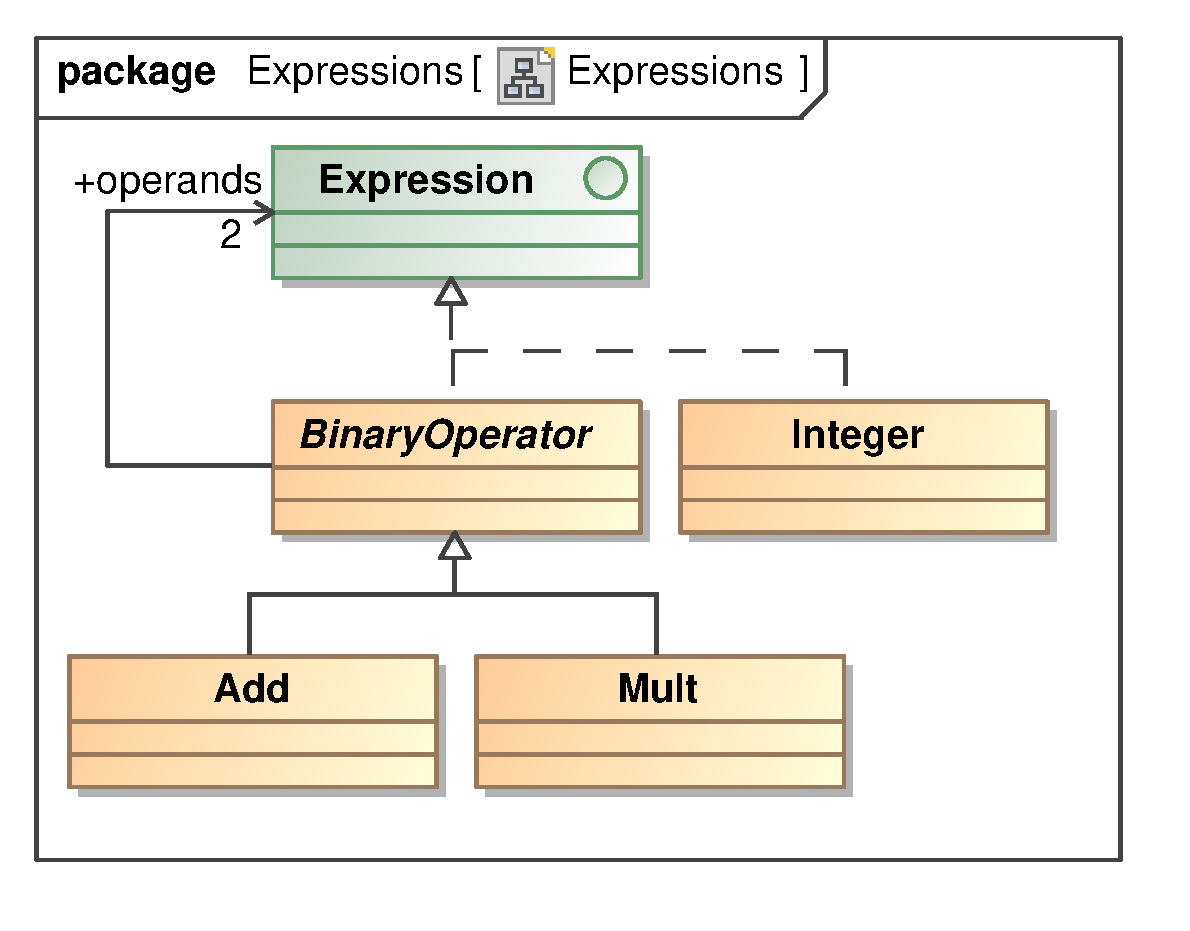
\includegraphics[width=.60\linewidth]{background/images/Expressions.eps} \\
  \caption{Diagrama de clases para el problema de las expresiones}
  \label{back:fig:expr}
\end{figure}
\begin{figure}[ht!]
  % Requires \usepackage{graphicx}
  \centering 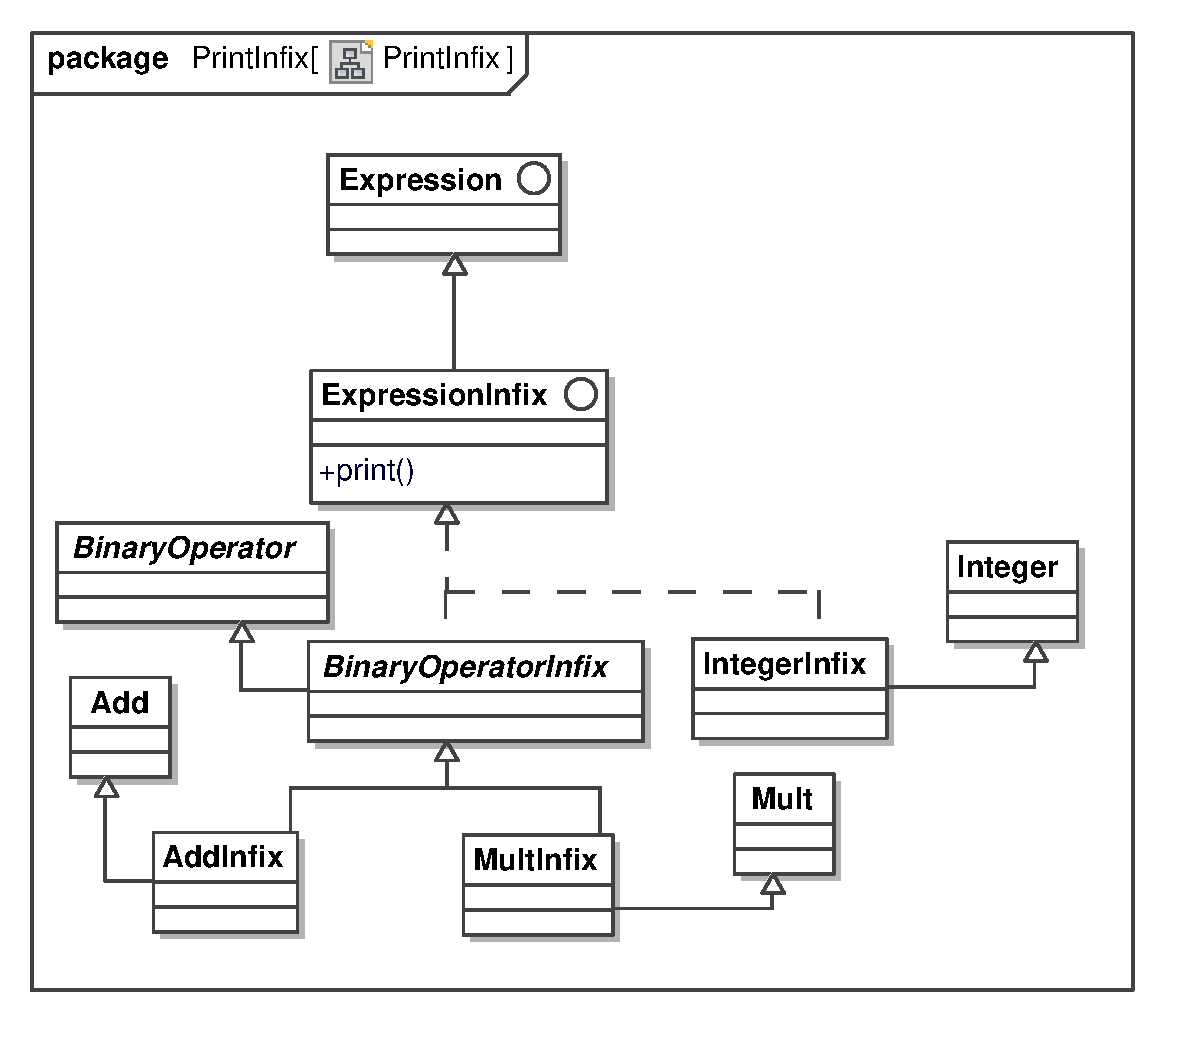
\includegraphics[width=.80\linewidth]{background/images/PrintInfix.eps} \\
  \caption{Diagrama de clases para la operaci�n de imprimir en formato infijo}
  \label{back:fig:printInfix}
\end{figure}
Tras trasladar estos diagramas a C\# se observan las carencias que posee un lenguaje orientado a objetos cuando implementamos un problema propio de la programaci�n orientada a caracter�sticas.\\
Por un lado he utilizado el mecanismo de herencia para a�adir funcionalidades a una clase existente, pero este mecanismo es jer�rquico, lo que hace que la clase hija herede toda la funcionalidad de su clase padre.
Por ejemplo, para crear una nueva configuraci�n que contenga las operaciones evaluar e imprimir en formato infijo se necesitar�a crear una nueva subclase que heredase de las clases que contienen las operaciones citadas anteriormente, pero esto no es posible, ya que C\#, como la mayor�a de los lenguajes orientados a objetos, solo permiten hacer uso de la herencia m�ltiple entre interfaces. Por lo tanto, por cada clase que se quiera heredar debemos crear una nueva interfaz que sea extendida por la clase a heredar y por la subclase que contendr� la nueva configuraci�n, a trav�s de esto y la creaci�n de objetos de las clases a heredar podremos acceder a los m�todos definidos por las interfaces, con lo que se consigue simular la herencia m�ltiple.\\
Pero el uso de esta t�cnica hace que, un incremento de funcionalidad representado por un conjunto de nuevas subclases que heredan de un conjunto de clases superiores, no sea posible manejarlo consistentemente como una unidad encapsulada. La insuficiente unidad de encapsulaci�n, deriva en un problema de complejidad en el manejo de la selecci�n de caracter�sticas para la composici�n. Aun cuando, las clases separadas en paquetes pertenezcan a una misma caracter�stica, es necesario seleccionar clases concretas que van a ser usadas en un producto espec�fico.
Otro problema es el manejo de las dependencias, ya que la herencia tradicional obliga a que las clases y subclases tengan diferentes nombres. Por lo tanto, las referencias a las clases concretas deben ser actualizadas. A mayor n�mero de caracter�sticas en una l�nea de productos, las relaciones entre clases concretas se complican potencialmente, lo que resulta una situaci�n indeseable. Esto incrementa la complejidad en las relaciones y dependencias entre clases.
% - Cuentas el ejemplo de las expresiones
% - Muestras la soluci�n en C#.

\subsubsection{Conclusiones}

Tras analizar el problema con un lenguaje orientado a objetos como es C\# se podr�a determinar que ser�a deseable encontrar en un lenguaje de programaci�n que estuviese orientado a caracter�sticas para obtener f�cilmente diferentes versiones de una misma aplicaci�n con la simple combinaci�n de diferentes conjuntos de caracter�sticas. Obviamente no todas las combinaciones ser�n v�lidas, por lo tanto, un lenguaje orientado a caracter�sticas deber�a de intentar asegurarse de que el resultado de la composici�n produce una aplicaci�n segura y bien configurada.
Con lo citado anteriormente, vamos a identificar una serie de caracter�sticas deseables que deber�amos encontrar en un lenguaje orientado a caracter�sticas:\\\\
\emph{Extensibilidad a trav�s de la adici�n y la substituci�n}\\
Como ya hemos comentado, una caracter�stica es normalmente considerada como un incremento en la funcionalidad de un programa. Por lo tanto, los lenguajes orientados a caracter�sticas deben proveer mecanismos para a�adir nuevas funcionalidades a una existente. En los lenguajes orientados a objetos, la extensi�n es realizada a trav�s de la herencia, pero �sta es adecuada cuando queremos extender una sola clase, pero com�nmente, las caracter�sticas necesitan ser extendidas por varias clases al mismo tiempo.
Adem�s la extensibilidad no siempre se alcanza por adici�n, en ocasiones es necesario el uso de la substituci�n. En los lenguajes orientados a objetos la substituci�n es llevada a trav�s de m�todos de sobre escritura (override en ingl�s).\\\\
\emph{Encapsulaci�n de caracter�sticas}\\
Todas las extensiones pertenecientes a una caracter�stica concreta deben ser a�adidas de una forma at�mica. Por lo tanto, los lenguajes orientados a caracter�sticas deber�an proveer de mecanismo para agrupar y encapsular los m�dulos pertenecientes a una misma caracter�stica. Por otra parte, estos m�dulos deber�an poderse compilar independientemente.\\\\
\emph{Composici�n a nivel de caracter�stica}\\
Productos espec�ficos, o configuraciones de una descomposici�n orientada a caracter�sticas, son obtenidos por la selecci�n y composici�n de unas caracter�sticas espec�ficas. Por lo tanto, ser�a deseable que un lenguaje orientado a caracter�sticas tuviese construcciones del lenguaje para producir un producto en particular. Esto deber�a ser realizado a nivel de caracter�stica, especificando que caracter�sticas deber�an ser incluidas, en lugar de tener que especificar los elementos individuales de cada caracter�stica.\\\\\\
\emph{Composici�n de caracter�sticas comprobando la coherencia}\\
No todas las combinaciones de caracter�sticas son v�lidas. Por lo tanto, un lenguaje orientado a caracter�sticas deber�a detectar las restricciones, evitando as� la implementaci�n de configuraciones no v�lidas y manejar autom�ticamente las dependencias en la medida de lo posible.

\subsection{Ventajas de los lenguajes orientados a caracter�sticas}
Los lenguajes orientados a caracter�sticas nos otorgan una mayor flexibilidad, ya que nos permiten que clases individuales puedan ser compuestas por un conjunto de caracter�sticas, por tanto son especialmente recomendados para utilizarlos con las l�neas de producci�n software.\\
Para estudiar las ventajas de los lenguajes orientados a caracter�sticas se trabajar� con CaesarJ que es un lenguaje de programaci�n basado en Java, que nos proporciona una mayor modularidad y el desarrollo a trav�s de componentes reusables.Para ello trabaja con conceptos como clases y paquetes en una �nica entidad, llamada familia de clases, que constituye unidades de encapsulamiento adicional para agrupar clases relacionadas. Una familia de clases tambi�n es, en s� misma una clase. As� mismo, se introduce el concepto de clases virtuales, que son clases internas (de familias de clases) propensas a ser refinadas a nivel de subclases. En el refinamiento de una clase virtual, impl�citamente se hereda de la clase que refina, por lo que tambi�n esto es visto como una relaci�n adjunta. Tambi�n, en un refinamiento pueden ser a�adidos nuevos m�todos, campos, relaciones de herencia y sobreescritura de m�todos. Puesto que en cada familia de clases, las referencias a las clases virtuales siempre apuntar�n al refinamiento m�s espec�fico. Esto significa que, por medio de las clases virtuales se aplica sobre escritura de m�todos, permitiendo redefinir el comportamiento de cualquier subclase de una familia de clases.\\
En t�rminos de programaci�n orientada a caracter�sticas, cada funcionalidad es modelada como una familia de clases. Mientras que los componentes y objetos del dominio espec�fico, son correspondidos por sus clases virtuales. As� mismo, las clases virtuales pueden ser declaradas como clases abstractas, lo que habilita la definici�n de interfaces en la implementaci�n modular de caracter�sticas.\\\\
Para hacer uso de lo citado anteriormente y ver su beneficio con las l�neas de producci�n software se ha vuelto a utilizar el ya comentado problema de las expresiones de la subsecci�n anterior. Pero en este caso, el dise�o cambia significativamente debido a la caracter�sticas expuestas de CaesarJ.\\
Por un lado en la figura \ref{back:fig:caesarJExpressions} se muestra que por cada operaci�n, tenemos una familia de clases, siendo la familia de clases que encapsula a todas las dem�s, la denominada \imp{Expressions}. �sta tiene la estructura de clases representado en la figura \ref{back:fig:expr}, y cada familia de clases lo que hace es redefinir las clases virtuales de \imp{Expressions} con las operaciones necesarias en cada caso.\\
\begin{figure}[ht!]
  % Requires \usepackage{graphicx}
  \centering 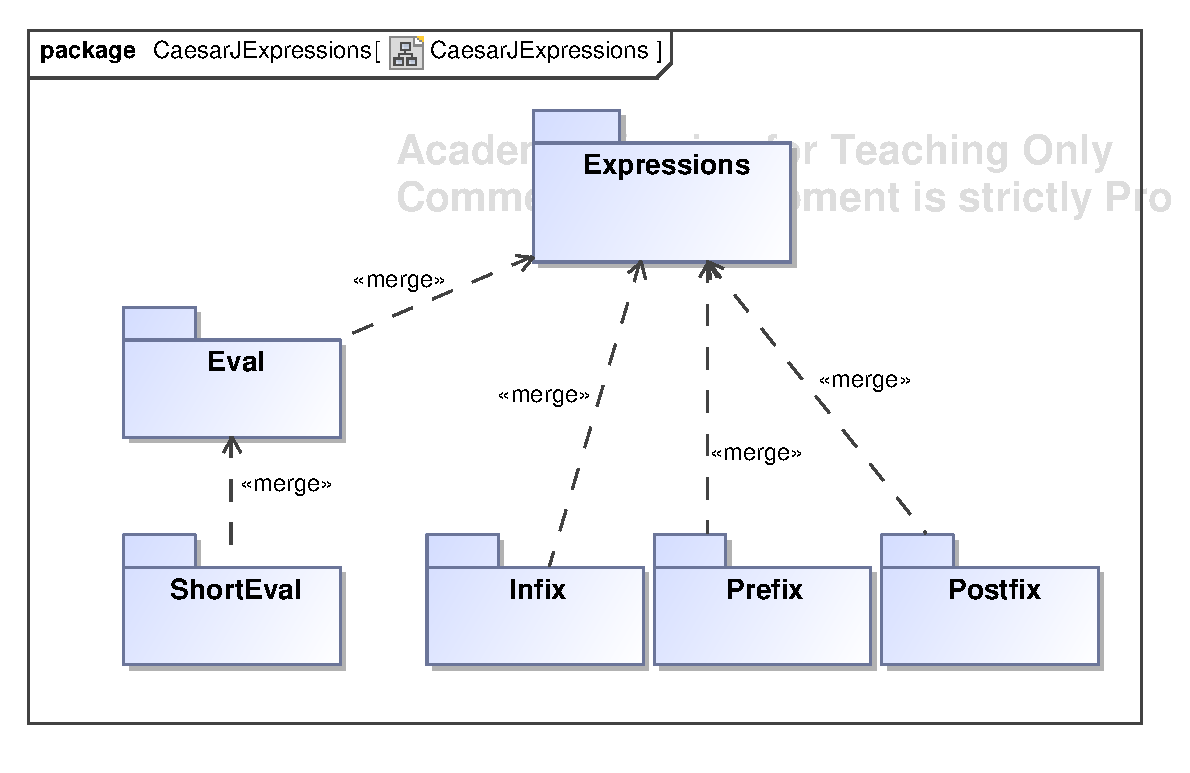
\includegraphics[width=.60\linewidth]{background/images/CaesarJExpressions.eps} \\
  \caption{Dise�o para resolver el problema de las expresiones con CaesarJ}
  \label{back:fig:caesarJExpressions}
\end{figure} 
\begin{figure}[ht!]
\begin{center}
\begin{footnotesize}
\begin{verbatim}
00 import eval.Eval;
01 import printPostfix.PrintPostfix;
02 import printInfix.PrintInfix;
03 import printPrefix.PrintPrefix;
04 public cclass EvalInfix extends PrintPrefix & Eval {}
\end{verbatim}
\end{footnotesize}
\end{center}
\caption{Configuraci�n que incluye las operaciones de evaluar e imprimir en formato infijo con CaesarJ}
\label{back:fig:codCaesarJ}
\end{figure}

Para realizar configuraciones, �nicamente se tiene que crear una nueva clase que extienda a las caracter�sticas que se deseen.A modo de ejemplo,la figura \ref{back:fig:codCaesarJ} muestra el c�digo necesario para crear una nueva configuraci�n que contenga las operaciones de impresi�n en formato posfijo y evaluaci�n de una expresi�n.Con todo esto, vemos como CaesarJ otorga un gran nivel de encapsulamiento y de reusabilidad de los componentes.

% P�rrafo introducci�n
% Introducci�n CaesarJ
% Ejemplo en CeasrJ, resaltando ventajas

\section{Clases Parciales C\#}
Las clases parciales C\# \cite{albahari:2010} nos permiten dividir la implementaci�n de una clase, estructura o interfaz en varios archivos de c�digo fuente. Cada fragmento representa una parte de la funcionalidad global de la clase. Todos estos fragmentos se combinan en tiempo de compilaci�n para crear una �nica clase, la cual contiene toda la funcionalidad especificada en las clases parciales. Por lo tanto,las clases parciales C\# pueden utilizarse como un mecanismo adecuado para implementar caracter�sticas, dado que cada incremento en funcionalidad para una clase se podr�a encapsular en una clase parcial separada.\\\\
Para poder ser compiladas y agrupadas en una sola clase, todas las clases parciales deben pertenecer al mismo espacio de nombres, poseer la misma visibilidad y deben ser declaradas con el indicador clave partial. En C\#, un espacio de nombre es simplemente empleado para agrupar clases relacionadas y evitar conflictos de nombres. Para especificar los archivos C\# que deben ser incluidos en una compilaci�n, se emplea un documento XML que contiene informaci�n acerca del proyecto y que especifica que ficheros deben ser compilados para generar el proyecto. Por lo tanto, es posible incluir y excluir f�cilmente la funcionalidad encapsulada dentro de una clase parcial simplemente a�adiendo o eliminando dicha clase parcial de este fichero XML.\\\\
Para ilustrar lo dicho anteriormente, se ha vuelto a utilizar el problema de las expresiones implement�ndolo con clases parciales. La figura \ref{back:fig:partialClass} muestra como hemos excluido de la compilaci�n la caracter�stica que representa la operaci�n de imprimir una expresi�n en formato infijo.
Este mecanismo de clases parciales permite a�adir o compartir funcionalidad entre un conjunto de clases que no precisan estar relacionadas mediante ning�n tipo de relaci�n jer�rquica, tal como ocurre con la herencia.\\
Por lo tanto, algunos autores (Laguna et al, 2007) sostienen que, las clases parciales C\# representan una alternativa a la herencia m�ltiple para manejar variabilidad relacionada programaci�n orientada a caracter�sticas.
\begin{figure}[!t]
\begin{center}
\begin{footnotesize}
\begin{verbatim}
01    <itemgroup>
02    <!--Eval-->
03    <Compile Include="Eval\Add.cs" />
04    <Compile Include="Eval\IExpressionsEval.cs" />
05    <Compile Include="Eval\IExpressions.cs" />
06    <Compile Include="Eval\Integer.cs" />
07    <Compile Include="Eval\Mult.cs" />
08    <!--Infix-->
09    <!--<Compile Include="Infix\Add.cs" />
10    <Compile Include="Infix\IExpressionInfix.cs" />
11    <Compile Include="Infix\IExpressions.cs" />
12    <Compile Include="Infix\Integer.cs" />
13    <Compile Include="Infix\Mult.cs" />-->
14    ...
15    </itemgroup>
16    </Project>
\end{verbatim}
\end{footnotesize}
\end{center}
\caption{Implementaci�n del archivo XML que guarda la informaci�n para la compilaci�n}
\label{back:fig:partialClass}
\end{figure}

% Qu� hace esto aqu�

% Explicar que son brevemente, y ejemplo usando las expresiones



% Cap�tulo 3: Definici�n y Planificaci�n del Proyecto
%==================================================================%
% Author : Perez Ruiz, Alejandro                                   %
% Version: 1.0, 16/03/2011                                         %                   %                                                                  %
% Memoria del Proyecto Fin de Carrera                              %
% Cap�tulo Planificacion, Archivo ra�z                             %
%==================================================================%

\chapterheader{Definici�n y Planificaci�n del Proyecto}{Definici�n y Planificaci�n del Proyecto}

\label{chap:planificacion}

% Introducci�n al cap�tulo

\chaptertoc

\section{Caso de Estudio: Hogares Inteligentes Automatizados}

% Resumir lo que aparece en diversos documentos
El objetivo de estos hogares es el aumento de la comodidad y seguridad de sus habitantes, as� como hacer un uso m�s eficiente de la energ�a consumida. Se ha elegido este dominio por ser un dominio donde el uso de un enfoque basado en L�neas de Productos Software se hace casi imperativo, debido a la gran variabilidad existente en estos productos. Esta variabilidad se debe tanto a motivos de hardware, dado que los dispositivos a ser controlados e interconectados pueden variar enormemente, como funcionales, dado que existen multitud de funcionalidades que se pueden ofrecer de manera opcional o alternativa al usuario, no siendo necesario que un determinado hogar las posea todas ellas.

Los ejemplos m�s comunes de tareas automatizadas dentro de un hogar inteligente son el control de luces, ventanas, puertas, persianas, calefacci�n, etc. Del mismo modo, se puede incrementar la seguridad de sus habitantes mediante sistemas automatizados de vigilancia y alertas de potenciales situaciones de riesgo, tales como detecci�n de humos o ventanas abiertas cuando se abandona el hogar.

Para el funcionamiento de los hogares los dispositivos de control inteligente leen datos de los sensores, procesan estos datos, y activan los actuadores, si fuese necesario. Para algunas tareas de control y automatizaci�n los dispositivos de control inteligentes act�an aut�nomamente.

La puerta de enlace (\emph{Gateway}, en ingl�s) es el servidor central del hogar inteligente. �ste realiza el procesado y el almacenamiento de los datos requeridos para las aplicaciones. Los usuarios(tanto residentes como t�cnicos), pueden acceder a los servicios ofrecidos a trav�s de la puerta de enlace o a trav�s de otras interfaces de usuario disponibles.

El presente proyecto se centrar� en el desarrollo de un hogar inteligente como una l�nea de productos software, con un n�mero variable de plantas y habitaciones. El n�mero de habitaciones por planta es tambi�n variable. La arquitectura de la l�nea de productos implementa varios servicios, clasificados en funciones b�sicas y complejas, que son descritas a continuaci�n.


Las \emph{funciones b�sicas} son:
\begin{enumerate}
\item \emph{Control autom�tico de luces:} Los habitantes del hogar deben ser capaces de encender, apagar y ajustar la intensidad de las diferentes luces de la casa. El n�mero de luces por habitaci�n es variable. El ajuste debe realizarse especificando un valor de intensidad.
\item \emph{Control autom�tico de puertas:} Las puertas pueden abrirse autom�ticamente. Adem�s, el control de acceso de algunas puertas puede ser necesario.
\item \emph{Control autom�tico de ventanas:} Los residentes tienen que ser capaces de controlar las ventanas autom�ticamente.Adem�s, si la ventana tiene persianas, �stas deben ser desenrolladas o enrolladas autom�ticamente.
\item \emph{Control autom�tico de temperatura:} El usuario ser� capaz de ajustar la temperatura de la casa.La temperatura podr� ser manejada en grados Celsius o Fahrenheit.
\end{enumerate}

Las \emph{funciones complejas} son:

\begin{enumerate}
\item \emph{Control inteligente de energ�a:} Esta funcionalidad trata de coordinar el uso de ventanas y aparatos para regular la temperatura interna de la casa, de manera que se haga un uso m�s eficiente de la energ�a consumida por parte de los aparatos de fr�o/calor. Por ejemplo, si se recibe la orden de calentar la casa, a la vez que se activan los radiadores se cerrar�n las ventanas de la casa para evitar las p�rdidas de calor.
\item \emph{Control inteligente de luces:} Las luces deber�n autom�ticamente apagarse/encenderse dependiendo de diversos factores. Si no hay luz natural fuera de la casa, las luces deber�n autom�ticamente encenderse. Cada vez que un habitante entre a una habitaci�n donde no haya iluminaci�n suficiente, las luces autom�ticamente se encender�n, a menos que la habitaci�n est� en modo "sleep". Este modo previene el alumbrado autom�tico de una habitaci�n,en el caso de que alguien estuviese durmiendo.
\item \emph{Presencia simulada:} Para evitar posibles robos, cuando los habitantes dejen la casa por un periodo largo de tiempo, la presencia de personas podr� ser simulada. Hay dos opciones(no exclusivas entre ellas):
    \begin{enumerate}
    \item Simulaci�n de las luces: Las luces podr�n ser apagadas/encendidas para simular presencia. Se usar� un esquema semi-aleatorio, por ejemplo el esquema variar� cada d�a acorde a unos parametros aleatorios, pero las luces no ser�n apagadas/encendidas sin sentido, ser�n encendidas m�s por la tarde/noche que durante el d�a.
    \item Simulaci�n de persianas: Las persianas ser�n subidas y bajadas, acorde con un esquema semi-aleatorio.Por ejemplo,las persianas de los dormitorios principales ser�n bajadas por la noche y subidas por la ma�ana,y las otras habitaciones, algunas noches se bajar�n y otras noches no.
    \end{enumerate}
\item \emph{Detecci�n de incendios:} Si alguno de los sensores instalados por las habitaciones detecta un fuego, se proceder� activar los aspersores de agua instalados en la habitaci�n, adem�s de activar la alarma de fuego.
\end{enumerate}

Cada una de estas funciones son opcionales. Las personas interesadas en adquirir el sistema podr�n seleccionar el numero de funciones que ellos deseen.

\section{Planificaci�n}

% Imagen a una sola columna
\begin{figure}[!tb]
  % Requires \usepackage{graphicx}
  \centering \includegraphics[width=.25\linewidth]{planificacion/images/gantt.eps} \\
  \caption{Diagrama de dependencias entre tareas}
  \label{fig:gantt}
\end{figure}

% Imagen a dos columnas
%\begin{figure*}[!tb]
%  % Requires \usepackage{graphicx}
%  \centering \includegraphics[width=\linewidth]{figures/gantt.eps} \\
%  \caption{(Left) Invalid configuration (Right) Valid configuration}
%  \label{fig:contexts}
%\end{figure*}

La figura~\ref{fig:gantt} muestra




% Cap�tulo 4: Domain Engineering
%%==================================================================%%
%% Author : P�rez Ruiz, Alejandro                                   %%
%% Author : S�nchez Barreiro, Pablo                                 %%
%% Version: 1.1, 14/06/2011                                         %%
%%                                                                  %%
%% Memoria del Proyecto Fin de Carrera                              %%
%% Cap�tulo Domain Engineering, Archivo ra�z                        %%
%%==================================================================%%

\chapterheader{Ingenier�a del Dominio}{Ingenier�a del Dominio}
\label{chap:domain}

Este cap�tulo se describe la fase de \emph{ingenier�a del dominio} (en ingl�s, \emph{Domain Engineering}) de nuestra l�nea de productos software. Dentro de dicha fase, se detalla la definici�n de la arquitectura de la familia de productos y se detallan las iteraciones m�s relevantes de este proceso de desarrollo. Las otras iteraciones, por motivos de espacio y con objeto de no aburrir al lector con detalles irrelevantes, simplemente se omiten.

\chaptertoc

\section{Definici�n Arquitect�nica}

%%==================================================================%%
%% Author : P�rez Ruiz, Alejandro                                   %%
%% Author : S�nchez Barreiro, Pablo                                 %%
%% Version: 1.1, 16/01/2011                                         %%                                                                                    %%                                                                  %%
%% Memoria del Proyecto Fin de Carrera                              %%
%% Domain Engineering/Architecture                                  %%
%%==================================================================%%

Un hogar inteligente posee una serie de dispositivos que se descomponen en \emph{sensores} y \emph{actuadores}. Los \emph{sensores} son los encargados de obtener los datos del elemento al que pertenecen, como por ejemplo, los grados que hace en una habitaci�n, la apertura que tiene una ventana... Los \emph{actuadores} se encargan de ejecutar las ordenes, por ejemplo que una persiana se abra o se cierre, la calefacci�n se encienda a unos determinados grados...

Tanto los sensores como los actuadores se encuentran conectados a un dispositivo central que los coordina, el cual se conoce como \emph{puerta de enlace} (en ingl�s, \emph{Gateway}). Dicho Gateway se encarga de leer los datos de los sensores, procesarlos y enviar las ordenes adecuadas a los actuadores. De igual modo, el Gateway recibe ordenes de los usuarios que son ejecutadas por los actuadores para modificar los elementos de la casa.

%%=====================================================================%%
%% HECHO(Pablo): Aqu� hace falta una figura describiendo la            %%
%%              arquitectura                                           %%
%% http://www.google.es/imgres?imgurl=http://www.fancybread.com/blog/images//mediator.jpg&imgrefurl=http://www.fancybread.com/blog/post.cfm/mediator-pattern-applied-to-javascript&h=273&w=316&sz=25&tbnid=x1f5CI5WvMYNzM:&tbnh=101&tbnw=117&prev=/search%3Fq%3DMediator%2BPattern%26tbm%3Disch%26tbo%3Du&zoom=1&q=Mediator+Pattern&hl=es&usg=__ZG2xo8qDKX8sPv-uWS_mDcE-zQo=&sa=X&ei=MnL7TZLvNcWYhQfkrYizAw&ved=0CEcQ9QEwBQ
%%=====================================================================%%
Por tanto, tal como se ve en la Figura~\ref{domain:fig:mediator}, el dise�o de nuestra arquitectura es una aplicaci�n concreta del patr�n de dise�o \emph{mediador}~\cite{gamma:1994}, donde el \emph{Gateway} ejercer el papel de mediador, y los diferentes sensores y actuadores son los distintos elementos a coordinar. El objetivo de este patr�n es extraer y encapsular en una �nica clase la l�gica de coordinaci�n de un conjunto de objetos que necesitan interaccionar entre ellos siguiendo reglas de coordinaci�n de cierta complejidad. Al encapsular esta l�gica en un �nico objeto, denominado \emph{mediador} , el dise�o de los diferentes objetos que deben interactuar, en nuestro caso sensores y actuadores,  se simplifica, ya que estos elementos ahora s�lo tienen que notificar eventos al mediador y recibir notificaciones del mismo. Del mismo modo, cualquier cambio en la l�gica de coordinaci�n de estos objetos afecta solo a la clase \emph{Mediador}, el \emph{Gateway} en nuestro caso, en lugar de a los diferentes objetos que toman parte en la interacci�n.
\begin{figure}[!h]
 \centering
 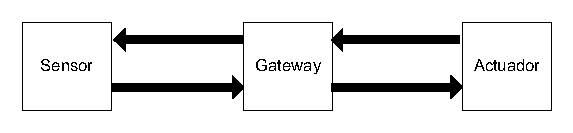
\includegraphics[width=.55\linewidth]{domainEngineering/images/Mediator.eps} \\
 \caption{Dise�o de la arquitectura a trav�s del patr�n de dise�o \emph{mediador}}
 \label{domain:fig:mediator}
\end{figure}

Adem�s de los sensores y actuadores, para que el usuario pueda controlar y visualizar el estado de los diversos dispositivos es necesario la creaci�n de una interfaz gr�fica que permita al usuario interactuar con el \emph{Gateway}.

Esta interfaz gr�fica tendr� que actualizar el estado de sus elementos cuando se producen cambios en los dispositivos. Para simplificar esta dependencia entre la interfaz gr�fica y el \emph{Gateway}, haremos uso del patr�n \emph{Observador}~\cite{gamma:1994} (\emph{Observer pattern}, en ingl�s). Para instanciar este patr�n, el \emph{Gateway} contendr� una lista por cada dispositivo que pueda ser observado. Los objetos interesados en ser notificados cada vez que dicho dispositivo cambie su estado se registrar�n o a�adir�n en dicha lista. De esta forma, cada vez que un dispositivo cambia de estado, el \emph{Gateway} notifica dicho cambio a todos los objetos registrados en la correspondiente lista de \emph{observadores}.

Finalmente, y dado que este proyecto no trabaja con actuadores y sensores reales, es necesario simular mediante software dichos dispositivos. Por ejemplo, deberemos simular variables tales como la temperatura percibida por los sensores, o el transcurso del tiempo del sistema. Para ello crearemos una interfaz gr�fica que juegue el papel de simulador, y permita al usuario interactuar con los dispositivos a simular as� como alterar diversas variables externas al sistema, como la temperatura.

Una vez definido el dise�o arquitect�nico b�sico, se desarrollan las iteraciones necesarias para completar la fase de ingenier�a del dominio. La siguiente secci�n describe los principios de dise�o seguidos para la construcci�n de dichas caracter�sticas. 

\section{Principios de Dise�o}
\label{domain:sec:pattern}

%%==================================================================%%
%% Author : P�rez Ruiz, Alejandro                                   %%
%% Author : S�nchez Barreiro, Pablo                                 %%
%% Version: 1.1, 14/06/2011                                         %%
%%                                                                  %%
%% Memoria del Proyecto Fin de Carrera                              %%
%% Domain Engineering/Interacion Dos                                %%
%%==================================================================%%

Para dise�ar nuestra l�nea de productos software seguimos un enfoque similar al de CaesarJ (cf.~\ref{back:subsec:foLanguages}), tratando de encapsular cada caracter�stica en una familia de clases.
La Figura~\ref{domain:fig:packageDiagram} muestra la descomposici�n en caracter�sticas de nuestro problema, as� como las dependencias entre las diferentes caracter�sticas. Siguiendo los principios de dise�o propuestos dentro del proyecto AMPLE~\cite{ample:d22}, cada familia de clases se representa como un paquete UML y las relaciones de herencia entre familias de clases como relaciones \emph{merge} entre paquetes.

\begin{figure}[!h]
 \centering
 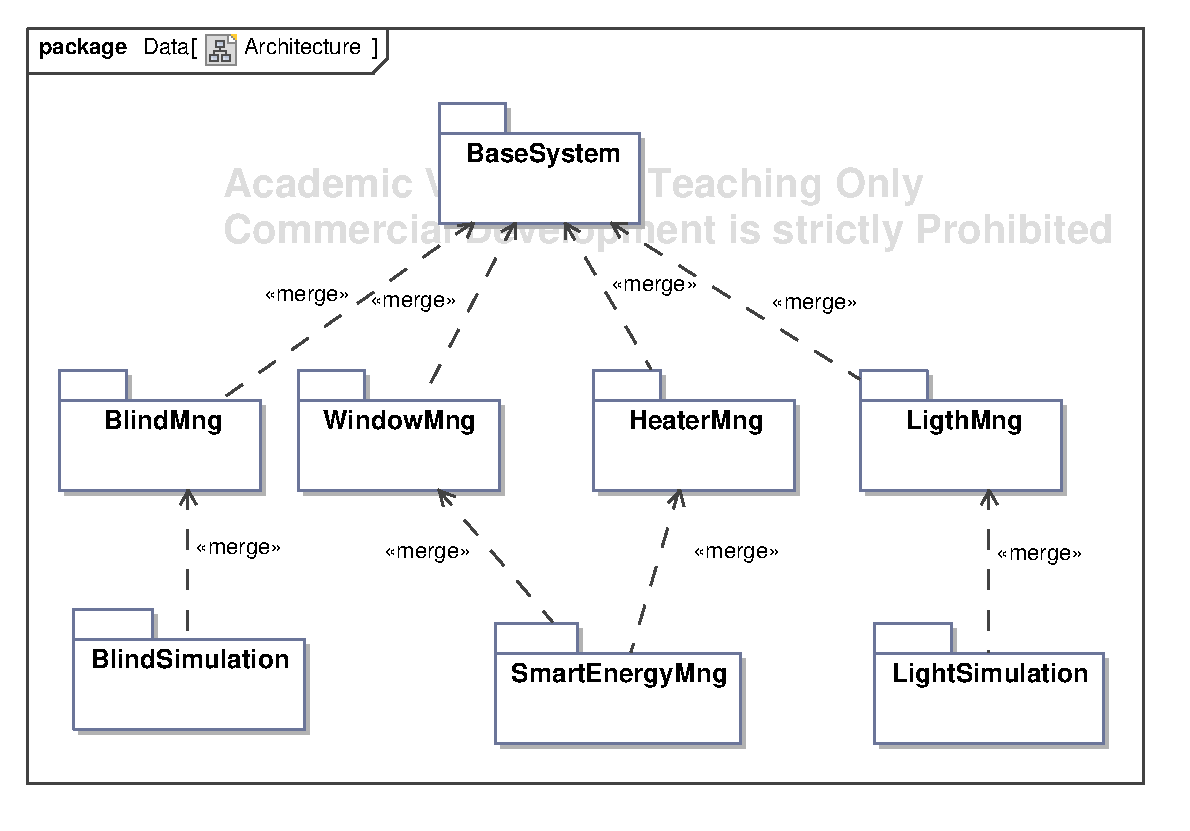
\includegraphics[width=.55\linewidth]{domainEngineering/images/packageDiagram.eps} \\
 \caption{Descomposici�n Orientada a Caracter�sticas de nuestra LPS}
 \label{domain:fig:packageDiagram}
\end{figure}

Para simular los mecanismos proporcionados por CaesarJ, usaremos las clases parciales de C\#. De esta forma, cada clase contenida en uno de los paquetes de la Figura~\ref{domain:fig:packageDiagram} se implementar� como una clase parcial que pueda ser extendida con nuevas funcionalidades en subsiguientes caracter�sticas. No obstante, el principal problema de este esquema es que las clases parciales, tal como ha sido identificado por~\cite{elio:2010},
no permiten la sobreescritura de m�todos. Este problema aparece cuando se da una situaci�n como la de la  Figura~\ref{domain:fig:override}.

%%====================================================================%%
%% HECHO(Pablo): Ajusta los tama�os para que quede bonito              %%
%%====================================================================%%
\begin{figure}[!h]
 \centering
 \includegraphics[width=.40\linewidth]{domainEngineering/images/overriding.eps} \\
 \caption{Problema de la sobreescritura con m�todos parciales C\#}
 \label{domain:fig:override}
\end{figure}

En este caso, la clase \imp{A} de la caracter�stica \imp{FeatureY} debe sobreescribir el m�todo \imp{aMethod()} de la versi�n de la clase \imp{A} para la caracter�stica \imp{FeatureX} con objeto de alterar su funcionalidad. Si la clase \imp{A} est� implementada como clase parcial de C\# en las caracter�sticas \imp{FeatureX} y \imp{FeatureY}, al intentar combinarlas el compilador reportar� un error indicando que existen m�todos con id�ntico perfil en clases parciales distintas. Este error se produce porque el compilador no soporta la fusi�n de m�todos o \emph{m�todos parciales}, lo cual es bastante l�gico. Dados dos m�todos con id�ntica cabecera, pero con implementaciones distintas, lo extra�o ser�a que el compilador supiese como fusionar dichas implementaciones de forma correcta.

Por tanto, hemos de idear un m�todo para poder sobreescribir m�todos. La soluci�n planteada se ilustra en la Figura~\ref{domain:fig:overrideSolution}. Dado que no podemos tener m�todos con id�ntico nombre y argumentos en diferentes clases parciales, cada m�todo correspondiente a una caracter�stica se precede con el nombre de la caracter�stica a la cual pertenece. Teniendo en cuenta que cada clase parcial pertenece a una caracter�stica diferente, si cada caracter�stica tiene un nombre �nico, nos aseguraremos de que no existir� colisi�n entre nombres de m�todos.

Cuando queremos crear un producto espec�fico, seguiremos la siguiente estrategia. Crearemos una nueva familia de clases que represente el producto final (\imp{aProduct}). Dicha familia de clases contendr� una clase parcial por cada clase distinta contenida en una caracter�stica seleccionada. Las clases contenidas en la familia de clases representando el producto espec�fico contendr�n un m�todo por cada m�todo distinto (sin considerar el prefijo del nombre que indica la caracter�stica a la cual pertenece). Por �ltimo, cada m�todo delegar� en la versi�n correspondiente a la versi�n m�s profunda de dicho m�todo en el �rbol de herencia entre familias de clases.

%%====================================================================%%
%% HECHO(Pablo): Ajusta los tama�os para que quede bonito              %%
%%====================================================================%%
\begin{figure}[!h]
 \centering
 \includegraphics[width=.40\linewidth]{domainEngineering/images/solution.eps} \\
 \caption{Soluci�n para el problema de la sobreescritura}
 \label{domain:fig:overrideSolution}
\end{figure}

Ilustramos dicha soluci�n con un ejemplo concreto, el cual se ilustra en la Figura~\ref{domain:fig:overrideSolution}. En dicha soluci�n, s�lo la caracter�stica \imp{FeatureX} debe incluirse dentro del producto concreto a construir. Tal como indica nuestro patr�n de soluci�n, creamos una familia de clases \imp{aProduct} para representar el producto concreto deseado. A continuaci�n, a�adimos la clase parcial \imp{A} a dicha familia de clases, por estar dentro de la caracter�stica \imp{FeatureX}. Seguidamente, a�adimos el m�todo \imp{aMethod} a la recientemente creada clase \imp{A}. Este m�todo delegar� en la operaci�n \imp{featureX\_aMethod}, por ser la versi�n correspondiente a este m�todo perteneciente a una caracter�stica seleccionada y que se encuentra m�s profunda en el �rbol de herencia entre familias de clases.

En las siguientes secciones describimos como siguiendo los principios de dise�o expuestos en esta secci�n, se han creado las iteraciones necesarias para crear el sistema base, controlar aparatos de fr�o/calor, las ventanas y el control inteligente de energ�a. Se han elegido estas interacciones, y no otras, por parecernos las m�s interesantes. Las otras se omiten por ser similares a �stas y por motivo de espacio.


\section{Iteraci�n 1: Sistema Base}

%%==================================================================%%
%% Author : P�rez Ruiz, Alejandro                                   %%
%% Author : S�nchez Barreiro, Pablo                                 %%
%% Version: 1.1, 14/06/2011                                         %%
%%                                                                  %%
%% Memoria del Proyecto Fin de Carrera                              %%
%% Domain Engineering/BaseSystem                                    %%
%%==================================================================%%

En la primera iteraci�n debemos definir la estructura b�sica del patr�n \emph{Mediador}. Adem�s, deberemos crear el esquema b�sico de la interfaz gr�fica, la cual deber� permitir controlar hogares con un n�mero de plantas y habitaciones variable. Adem�s la interfaz gr�fica deber� permitir la incorporaci�n de nuevas subinterfaces para el control de diversas funcionalidades, como por ejemplo, el control autom�tico de luces o ventanas. Los requisitos concretos que se han de satisfacer en esta iteraci�n se muestran en la Figura~\ref{plan:table:requisitos}.

%%====================================================================%%
%% NOTA(Pablo): Haz esta imagen m�s ancha que larga, m�s compacta y   %%
%%              m�s sim�trica                                         %%
%%====================================================================%%

\begin{figure}[!tb]
 \centering
 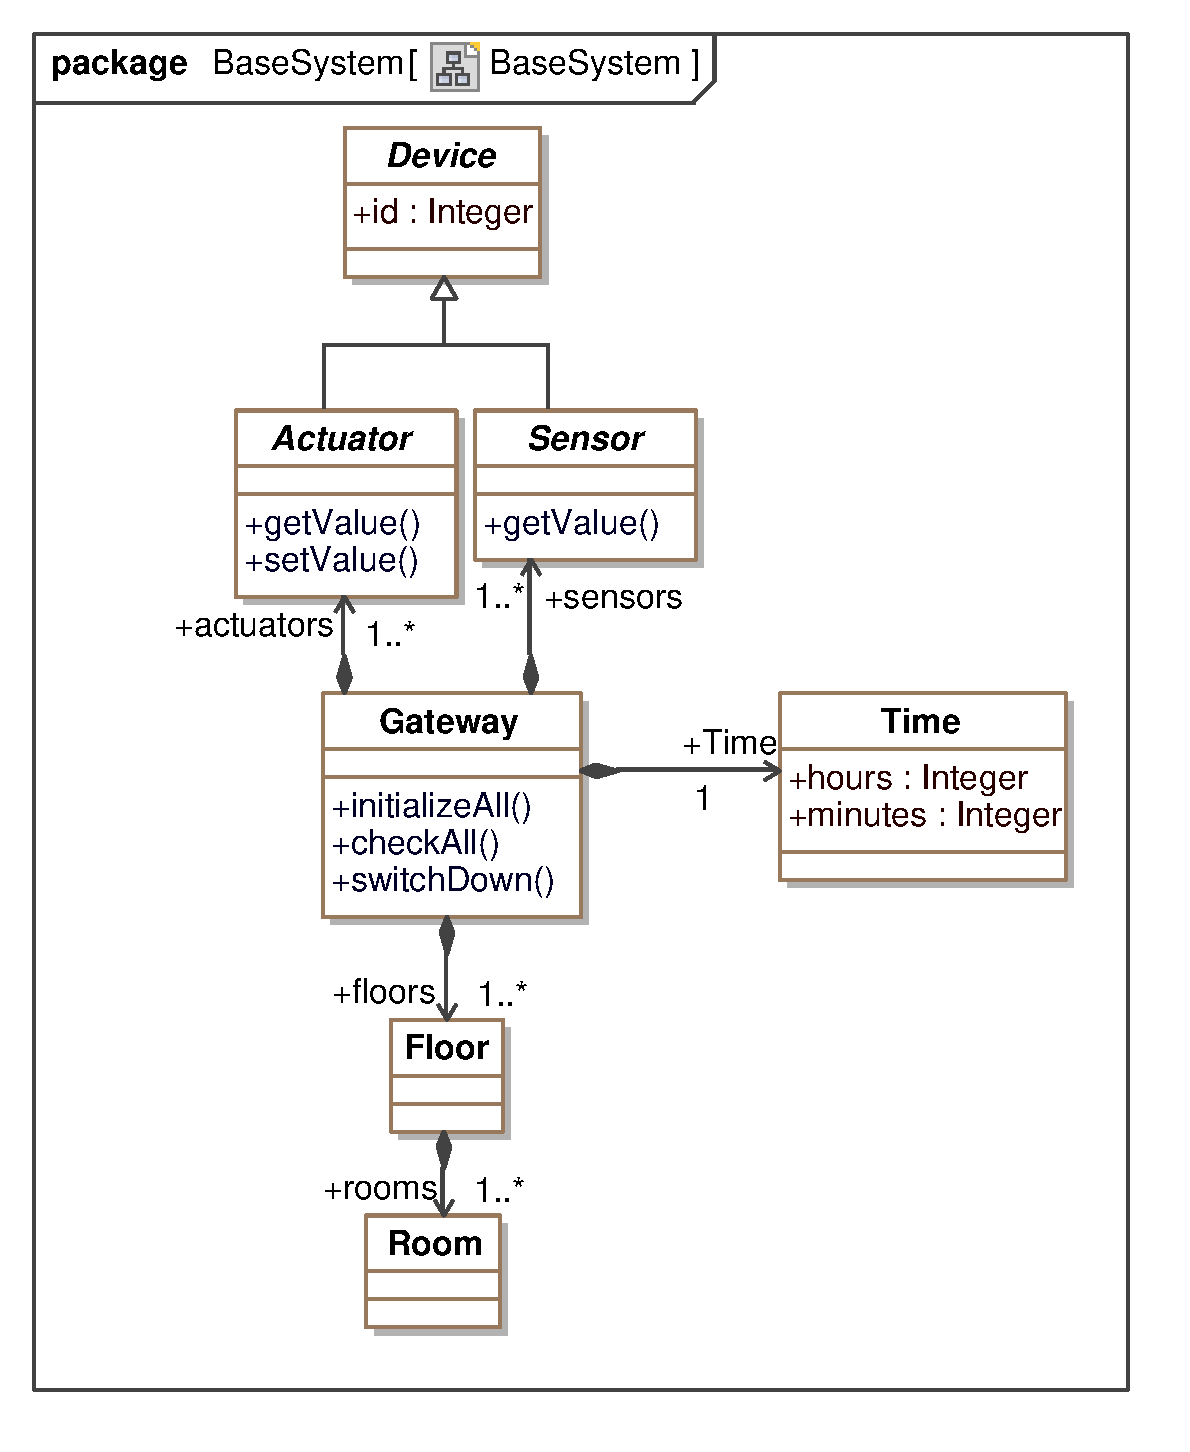
\includegraphics[width=.45\linewidth]{domainEngineering/Images/definicionArq.eps} \\
 \caption{Dise�o del sistema base}
 \label{domain:fig:defArq}
\end{figure}


La Figura~\ref{domain:fig:defArq} muestra el dise�o realizado para esta caracter�stica. Tal como se observa, el \emph{Gateway} posee una lista de plantas y a su vez cada planta contiene otra lista de las habitaciones que se encuentran en dicha planta. Se crea adem�s un objeto tiempo que se encarga de simular el transcurso del tiempo en el sistema. Todas las clases de la Figura~\ref{domain:fig:defArq} se implementar�n como clases parciales de C\#, de forma que puedan ser extendidas con nuevas funcionalidades en subsiguientes caracter�sticas.

%%====================================================================%%
%% NOTA(Pablo): Esto es redundante                                    %%
%%====================================================================%%
%%
%% Una parte importante del sistema son las interfaces gr�ficas que 
%% permitir�n al usuario interactuar con el Gateway. Se implementan 
%% dos, la primera de ellas permite al usuario actuar con el Gateway, 
%% mientras que la segunda har� el papel de simulador, ya que es 
%% necesario modificar algunos valores que deber�an ser alterados 
%% por elementos externos al propio sistema, tales como la temperatura 
%% actual de una habitaci�n o el tiempo,ya que el sistema no se 
%% encuentra conectado a dispositivos reales.
%%
%%====================================================================%%

A la par que la l�gica del sistema, debemos crear las interfaces gr�ficas que permitan al usuario interactuar con el sistema. No obstante, no debemos olvidar que estamos implementado una l�nea de productos software, por lo que todos los dise�os de las interfaces gr�ficas deben adaptarse a cualquier composici�n de caracter�sticas que haga un usuario.

\begin{figure}[!tb]
 \centering
 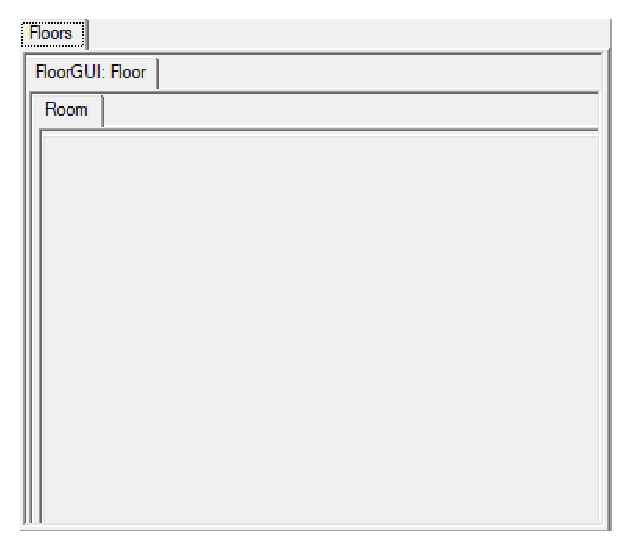
\includegraphics[width=.55\linewidth]{domainEngineering/Images/GUI.eps} \\
 \caption{Dise�o de la interfaz gr�fica de usuario}
 \label{domain:fig:gatewayGUI}
\end{figure}

Como punto de partida para el dise�o de las interfaces gr�ficas se ha utilizado la API para el desarrollo de aplicaciones gr�ficas que incluye .NET, denominada \emph{Windows Forms}~\cite{brown:2006}. Debido a que el n�mero de plantas y el
e habitaciones debe ser variable, la interfaz deber� permitir la visualizaci�n de una cantidad arbitraria de plantas. Adem�s, cuando una planta sea seleccionada se deber�n mostrar todas las habitaciones que contiene, y cada habitaci�n debe de poder contener diferentes caracter�sticas, tales como control de ventanas, persianas, luces, etc. Por todo lo citado anteriormente, se ha decidido utilizar un dise�o como el mostrado en la figura \ref{domain:fig:gatewayGUI}. En dicho dise�o, cada planta se representa como una pesta�a. Cada pesta�a que contiene habitaciones, representadas como pesta�as anidadas. A su vez, por cada caracter�stica seleccionada en una habitaci�n, se crear� una nueva pesta�a anidada, dentro de la pesta�a de cada habitaci�n.

%%====================================================================%%
%% NOTA(Pablo): Esto es demasuiado detalle irrelevante
%%====================================================================%%
%%
%% Con esta API para construir una interfaz gr�fica se deben a�adir 
%% controles a una forma e implementar respuestas a las acciones de los 
%% usuarios, tales como un click de rat�n o la pulsaci�n de una tecla. 
%% Un control se define como una interfaz de usuario que muestra datos 
%% o acepta datos de entrada. Por lo que lo primero que se debe pensar 
%% es en los controles que ser�n m�s adecuados para la ventana que 
%% contiene la interfaz gr�fica. 
%%
%%====================================================================%%

Siguiendo este mismo razonamiento, hemos creado el dise�o para la interfaz gr�fica del simulador. En el caso del sistema base, solo se encargar� de mostrar las plantas y habitaciones que se han creado, por lo que se vuelve a seleccionar un control que permita a�adir pesta�as tal y como se muestra en la figura \ref{domain:fig:simulatorGUI} y una tabla con el identificador de una habitaci�n, su nombre y la planta a la que pertenecen.

\begin{figure}[!tb]
 \centering
 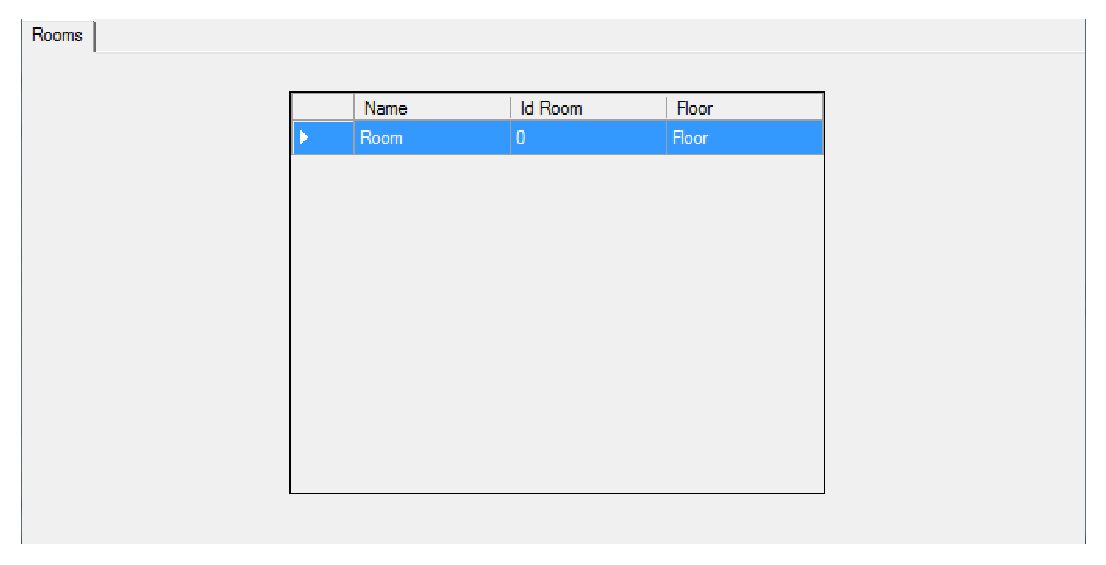
\includegraphics[width=.65\linewidth]{domainEngineering/Images/simulatorGUI.eps} \\
 \caption{Dise�o de la interfaz gr�fica para el simulador}
 \label{domain:fig:simulatorGUI}
\end{figure}

Para poder a�adir nuevas funcionalidades y caracter�sticas a ambas interfaces, �stas se implementan mediante clases parciales.

Una vez implementado todo el sistema base se realizaron una serie de test de prueba, cuyo objetivo era crear diferentes instancias del sistema para comprobar que tanto las plantas y habitaciones se creaban, a�ad�an y visualizaban en las interfaces gr�ficas correctamente.

Tras haber finalizado la implementaci�n del sistema base ya se tiene la infraestructura b�sica para poder crear nuevas caracter�sticas que extiendan y a�adan nuevas funcionalidades. La siguiente secci�n describe el proceso de desarrollo para la caracter�stica \emph{HeaterMng}, que se a�ade a este sistema base.


\section{Iteraci�n 2: Gesti�n de Sistemas de Control de Temperatura}

	%%==================================================================%%
	%% Author : P�rez Ruiz, Alejandro                                   %%
	%% Author : S�nchez Barreiro, Pablo                                 %%
	%% Version: 1.1, 14/06/2011                                         %%
	%%                                                                  %%
	%% Memoria del Proyecto Fin de Carrera                              %%
	%% Domain Engineering/Interacion Dos                                %%
	%%==================================================================%%

La caracter�stica de gesti�n de los sistemas de control de la temperatura  (\emph{HeaterMng}) deber�  permitir a los usuarios establecer el valor deseado para la temperatura (en grados Celsius). Los dispositivos de control de la temperatura funcionan como aparatos de fr�o/calor. De esta forma, si la temperatura especificada por el usuario es inferior a la actual, el dispositivo deber� enfriar la casa. En el caso opuesto, deber� calentarla.

%%=====================================================================%%
<<<<<<< .mine
%% NOTA(Pablo): Esto sobra
=======
%% NOTA(Pablo): Esto sobra                                          %%
>>>>>>> .r399
%%=====================================================================%%
%%
%% Para la situaci�n en la que la temperatura seleccionada por el
%% usuario coincida con la temperatura del lugar donde se encuentra el
%% calefactor, este �ltimo no entrar� en modo funcionamiento, por lo
%% que no consumir� energ�a.
%%
%%=====================================================================%%

Esta caracter�stica a�ade clases pare representar los nuevos dispositivos, m�s concretamente, \imp{Thermometer} y \imp{HeaterCtrl}, tal y como se ilustra en la Figura~\ref{domain:fig:heaterMngDesign}. Estos dispositivos extienden las clases abstractas \imp{Actuator} y \imp{Sensor}. Adem�s, se debe extender la clase \imp{Gateway} con nuevos m�todos y atributos para el control de estos nuevos dispositivos. A cada aparato de control de la temperatura se le asocia un term�metro en exclusiva, para realizar mediciones mas precisas.

\begin{figure}[!tb]
 \centering
 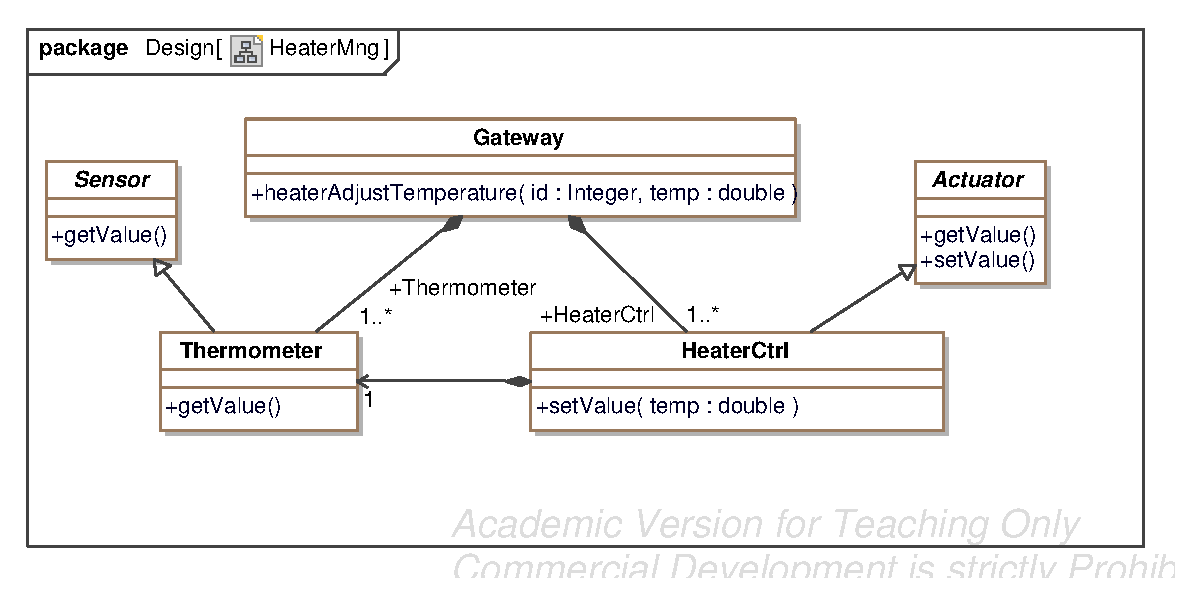
\includegraphics[width=.65\linewidth]{domainEngineering/Images/HeaterMngDesign.eps} \\
 \caption{Dise�o UML para la caracter�stica \emph{HeaterMng}}
 \label{domain:fig:heaterMngDesign}
\end{figure}

%%=====================================================================%%
%% NOTA(Pablo): Esto es trivial y no merece la pena contarlo
%%=====================================================================%%
%%
%% La principal acci�n que sostiene esta nueva caracter�stica es la de
%% modificar la temperatura de los calefactores por los usuarios del
%% sistema, por ello la figura \ref{domain:fig:secuenciaHeaterMng}
%% ilustra a trav�s de un diagrama de secuencia cuales son los pasos
%% de los mensajes necesarios para que la temperatura sea modificada.
%% Como ya se ha comentado en otras ocasiones en el diagrama de secuencia
%% se vuelve a observar como el Gateway es el mediador que se encarga de
%% transmitir los mensajes entre los distintos dispositivos.
%%
%%
%% \begin{figure}[!tb]
%5 \centering
%%  \includegraphics[width=.75\linewidth]
%%    {domainEngineering/Images/secuenciaHeaterMng.eps}%
%% \\
%% \caption{Diagrama de secuencia para modificar la temperatura.}
%%  \label{domain:fig:secuenciaHeaterMng}
%% \end{figure}
%%
%%=====================================================================%%

Tambi�n es necesario extender las dos interfaces gr�ficas que se implementaron en el sistema base. En el caso de la interfaz gr�fica para el control del \emph{Gateway}, a�adimos una nueva pesta�a a nivel global, para toda la casa, que permita encender o apagar todos los aparatos de control de la temperatura. En el caso de que los aparatos est�n conectados, se ofrecer� la opci�n de mostrar la temperatura deseada (ver Figura~\ref{domain:fig:GUIHeaterMng}). Pesta�as similares se a�aden a todas las plantas y habitaciones que contengan al menos un aparato de control de la temperatura.

%%=====================================================================%%
%% NOTA(Pablo): Con una captura vale. Aunque te haya costado trabajo,  %%
%%              esto no es del todo interesante. Deja la captura donde %%
%%              se ve todo                                             %%
%%=====================================================================%%

\begin{figure}[!tb]
 \centering
 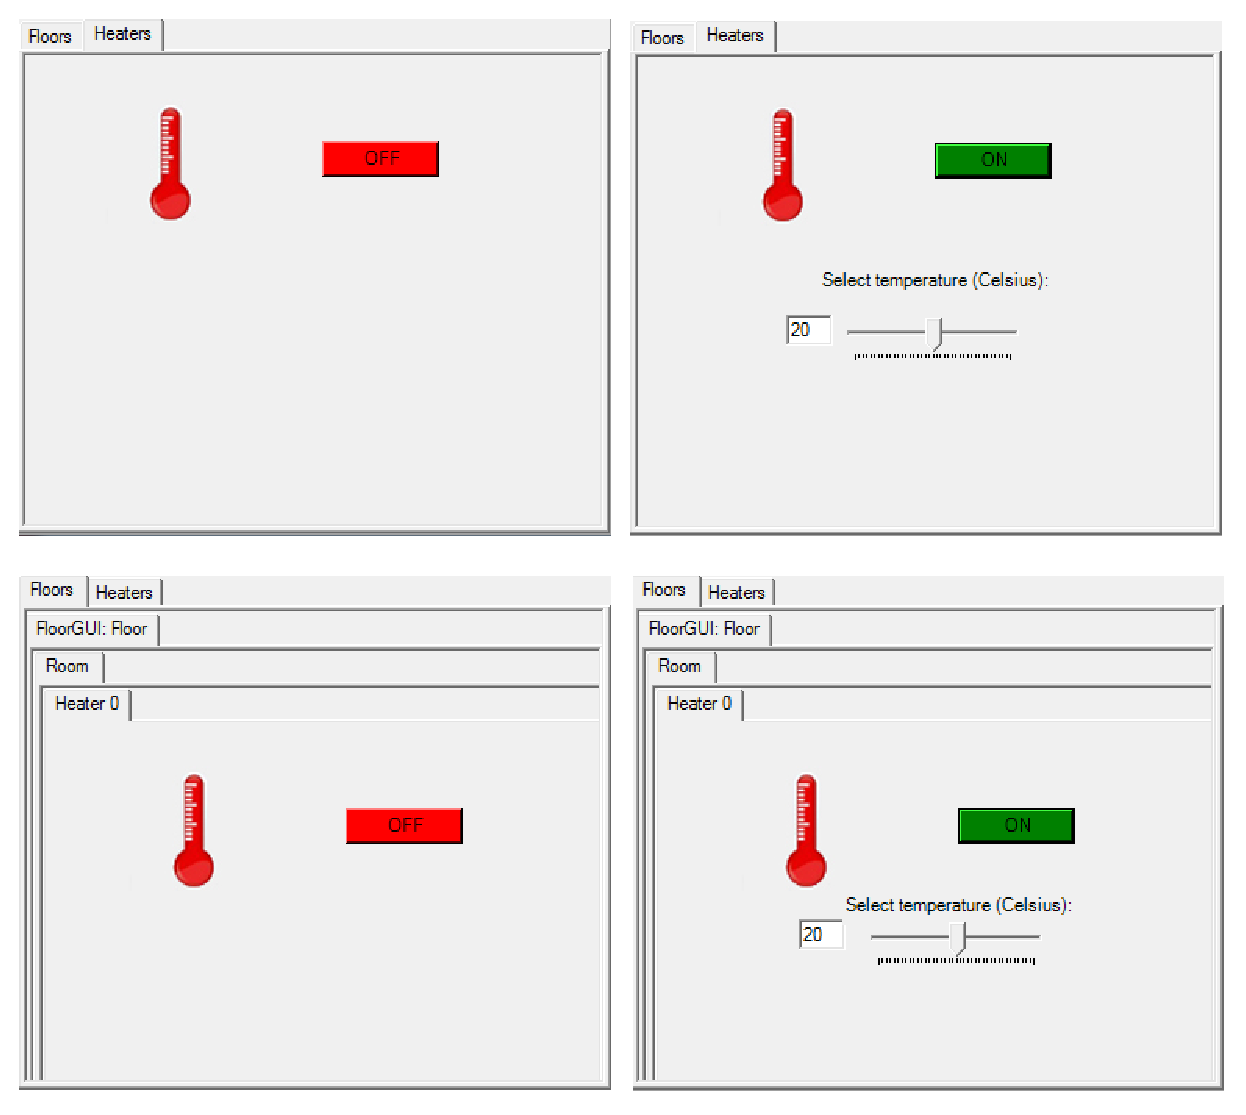
\includegraphics[width=.45\linewidth]{domainEngineering/Images/GUIHeaterMng.eps} \\
 \caption{Interfaz gr�fica de usuario con los elementos para el control de temperatura}
 \label{domain:fig:GUIHeaterMng}
\end{figure}

Por otro parte, tembi�n debemos extender la interfaz gr�fica del simulador. Por tanto, a�adimos una nueva pesta�a que muestre de forma tabular los diferentes aparatos de control de temperatura existentes en la casa as� como la informaci�n relacionada con los mismos de inter�s para observar el funcionamiento de la casa (ver Figura \ref{domain:fig:SimulatorHeaterMng}). Tambi�n se ofrece la posibilidad de cambiar el valor de la variable \emph{Temperatura} de cada term�metro, con objeto de analizar el comportamiento del hogar automatizado en diferentes situaciones.

\begin{figure}[!tb]
 \centering
 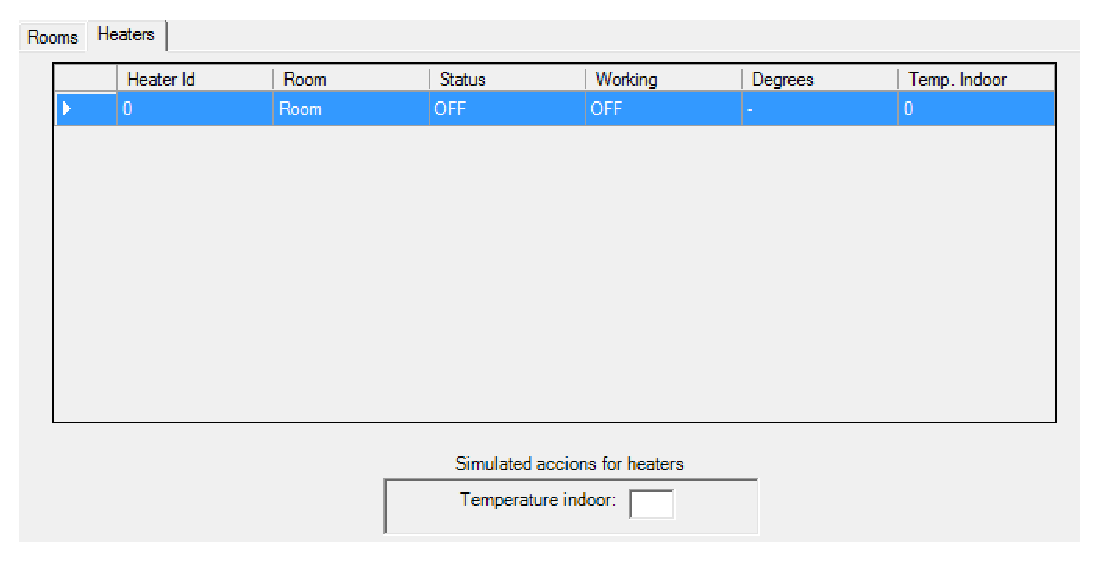
\includegraphics[width=.75\linewidth]{domainEngineering/Images/simulatorGUIHeaterMng.eps} \\
 \caption{Dise�o de la interfaz gr�fica de usuario para el simulador en la caracter�stica de \emph{HeaterMng}}
 \label{domain:fig:SimulatorHeaterMng}
\end{figure}

A continuaci�n, tanto el dise�o de la Figura~\ref{domain:fig:heaterMngDesign} como el de las interfaces mostradas en las Figuras~\ref{domain:fig:GUIHeaterMng} y~\ref{domain:fig:SimulatorHeaterMng}, se implementa usando los principios descritos en la Secci�n~\ref{domain:sec:pattern}. Por �ltimo, realizamos las pruebas de dicha implementaci�n. Los casos de prueba ejecutados se describen a continuaci�n:

\begin{enumerate}
\item Se han creado una serie de instancias del hogar inteligente con un n�mero de aparatos de control de la temperatura arbitrario y repartidos por distintas habitaciones.
\item Por cada instancia de un hogar concreto se ha verificado que se ejecutan correctamente las siguientes operaciones:
	\begin{enumerate}
		\item Es posible encender, apagar y modificar la temperatura de todos los aparatos de control de la temperatura a trav�s de la interfaz gr�fica de usuario. Dicho cambio se refleja adem�s en el simulador.
		%%=====================================================================%%
		%% NOTA(Pablo): Este caso de prueba no lo entiendo                     %%
		%%=====================================================================%%
		%% \item Por cada calefactor se modificar� su temperatura para que coincida con la de su term�metro, %% comprob�ndose que el calefactor cambie su modo de funcionamiento a sin consumo de energ�a.
		%%=====================================================================%%
		\item Es posible modificar la temperatura de los term�metros, y dicha alteraci�n afecta de forma correcta al modo de funcionamiento de los aparatos de control de la temperatura.
		\item Cuando el usuario modifica la temperatura deseada, los aparatos de fr�o/calor alteran su funcionamiento de la forma prevista.
	\end{enumerate}
\end{enumerate}




\section{Iteraci�n 3: Control Autom�tica de Ventanas}

%%==================================================================%%
%% Author : P�rez Ruiz, Alejandro                                   %%
%% Author : S�nchez Barreiro, Pablo                                 %%
%% Version: 1.1, 18/06/2011                                         %%
%%                                                                  %%
%% Memoria del Proyecto Fin de Carrera                              %%
%% Domain Engineering/Interacion Tres                               %%
%%==================================================================%%

La caracter�stica para en control autom�tico de ventanas tiene como principal requisito permitir a los usuarios abrir o cerrar una ventana con una determinada apertura (cf. Tabla~\ref{plan:table:requisitos}).

La Figura~\ref{domain:fig:designWindowMng} muestra el dise�o UML para esta caracter�stica, el cual se ha realizado siguiendo un proceso muy similar al de la secci�n anterior. Cada ventana tiene un sensor que se encargar� de enviar al \emph{Gateway} la apertura de dicha ventana; y un actuador, que abrir� o cerrar� la ventana cuando sea necesario. Este dise�o, al igual que anteriormente, se implementa usando clases parciales de C\#, siguiendo los principios establecidos en la Secci�n~\ref{domain:sec:pattern}.

%%=============================================================================================================%%
%% HECHO(Pablo): Esta imagen se puede hacer a�n m�s compacta.                                                   %%
%%=============================================================================================================%%
\begin{figure}[!tb]
 \centering
 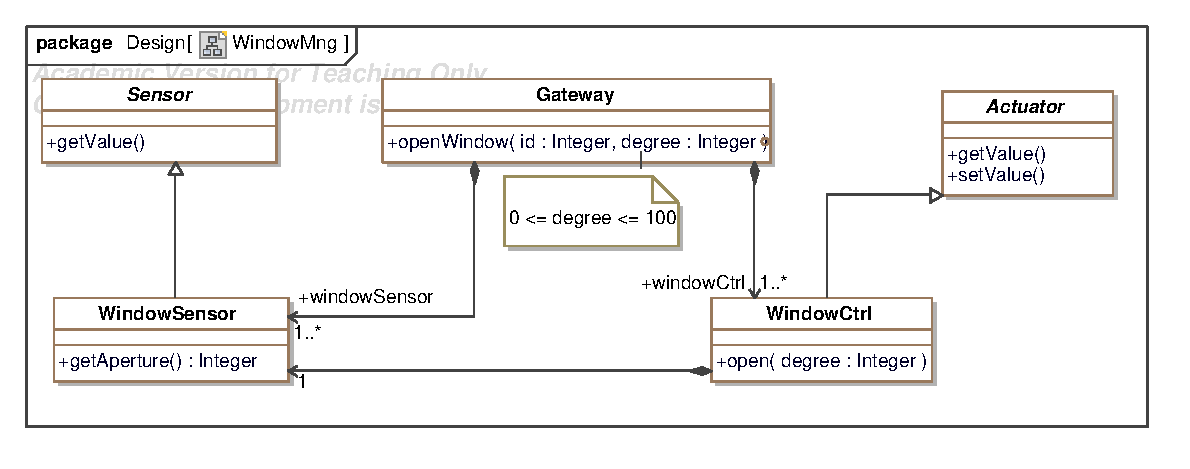
\includegraphics[width=.65\linewidth]{domainEngineering/Images/WindowMngDesign.eps} \\
 \caption{Dise�o de la caracter�stica \emph{WindowMng}.}
 \label{domain:fig:designWindowMng}
\end{figure}

las interfaces gr�ficas de usuario y de simulaci�n se extienden de un modo similar al de la iteraci�n anterior. La Figura~\ref{domain:fig:GUIWindowMng} muestra el aspecto visual de dichas interfaces.

%%=============================================================================================================%%
%% NOTA(Pablo): Todo esto se puede suprimir                                                                    %%
%%=============================================================================================================%%
%%
%% Para el caso de las dos interfaces gr�ficas se ha seguido un proceso similar que el utilizado en la
%% caracter�stica \emph{HeaterMng}, es decir, volviendo a definir las clases parciales que implementan a las
%% interfaces gr�ficas se a�aden nuevos controles del tipo pesta�a. De este modo las interfaces muestran un
%% dise�o como el representado en la figura \ref{domain:fig:GUIWindowMng}, en la cual en la parte superior de
%% la izquierda se ilustra la interfaz gr�fica del Gateway con la pesta�a global que controla todas las
%% ventanas, mientras que en la parte superior de la derecha se ilustra el dise�o destinado a controlar una
%% ventana espec�fica. En la parte inferior de la figura se muestra la interfaz gr�fica para el simulador.
%%
%%=============================================================================================================%%

%%=============================================================================================================%%
%% HECHO(Pablo): Quita una interfaz gr�fica para el control de ventanas e intenta que las dos te queden en una  %%
%%              misma l�nea                                                                                    %%     %%=============================================================================================================%%
\begin{figure}[!tb]
 \centering
 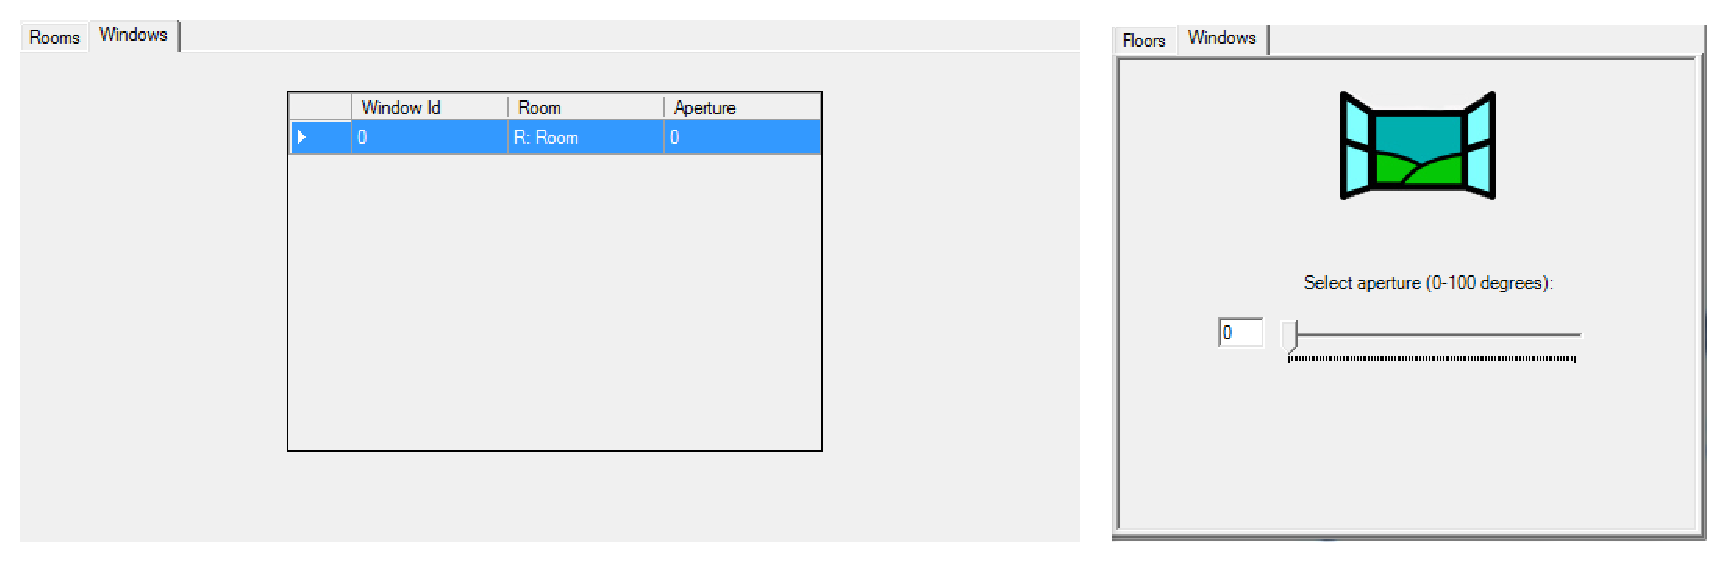
\includegraphics[width=.70\linewidth]{domainEngineering/Images/GUIWindowMng.eps} \\
 \caption{Dise�o de las interfaces gr�ficas para la caracter�stia \emph{WindowMng}}
 \label{domain:fig:GUIWindowMng}
\end{figure}

Al igual que en la iteraci�n anterior, una vez implementada la caracter�stica, se realizan una serie de pruebas para comprobar la correcci�n de la implementaci�n.

%%=============================================================================================================%%
%% NOTA(Pablo): Todo esto se puede suprimir                                                                    %%
%%=============================================================================================================%%
%%
%% Para las pruebas en esta caracter�stica se han realizado una serie de test, que han seguido el siguiente
%% procedimiento:
%%
%% \begin{enumerate}
%% \item Se han creado una serie de instancias del hogar inteligente con diferente n�mero de ventanas
%%         repartidas por distintas habitaciones.
%% \item Por cada instancia se realizan los siguientes casos de prueba:
%%    \begin{enumerate}
%%        \item Se modifica la apertura de las todas las ventanas, a trav�s de la pesta�a de
%%              control global de la caracter�stica, en la interfaz gr�fica del Gateway, y se comprueba
%%              en el simulador y en el propio Gateway.
%%        \item Por cada ventana se modifica su apertura, de modo individual a trav�s de su pesta�a
%%              espec�fica.
%%    \end{enumerate}
%% \end{enumerate}
%%
%%=============================================================================================================%%

La siguiente secci�n describe el proceso de desarrollo de la caracter�stica \emph{SmartEnergyMng}, la cual resulta d especial inter�s al tener que combinar de la forma adecuada la caracter�stica desarrollada en la secci�n actual con  la caracter�stica desarrolla en la secci�n anterior. 

\section{Iteraci�n 4: SmartEnergyMng}
\label{sec:domain:smartEnergy}



\section{Sumario}

En este cap�tulo se ha mostrado el proceso llevado a cabo para realizar la fase de ingenier�a de dominio en esta l�nea de productos software, en la cual se han utilizado las clases parciales de C\# como principal mecanismo para encapsular las caracter�sticas. No obstante, las clases parciales presentan alguna limitaci�n para encapsular correctamente, por lo que se han desarrollado y expuesto mecanismos para suplir estas limitaciones.

El siguiente cap�tulo mostrar� como utilizando la infraestructura desarrollada anteriormente, se pueden crear aplicaciones espec�ficas adaptadas a los requerimientos de los usuarios. 

% Cap�tulo 5: Domain Engineering
%==================================================================%
% Author : P�rez Ruiz, Alejandro                                   %
% Version: 1.0, 16/03/2011                                         %                                                                                    %                                                                  %
% Memoria del Proyecto Fin de Carrera                              %
% Cap�tulo Application Engineering, Archivo ra�z                   %
%==================================================================%

\chapterheader{Application Engineering}{Application Engineering}

\label{chap:application}

% Introducci�n al cap�tulo
La ingenier�a de aplicaci�n es un proceso en el cual, las aplicaciones de una l�nea de productos se construyen a trav�s de los artefactos creados en la fase de ingenier�a de dominio y la explotaci�n de la variabilidad de las l�neas de producto software \cite{pohl:2005}.
Los principales objetivos de la ingenier�a de aplicaci�n son: alcanzar un nivel tan alto como sea posible de reutilizar los elementos del dominio cuando se definan y desarrollen aplicaciones de la l�nea de productos y  explotar la variabilidad y los elementos comunes de la l�nea de productos software durante el desarrollo de aplicaciones. Por lo que este cap�tulo presentar� al lector el proceso seguido para conseguir reutilizar y componer los elementos creados en la fase de ingenier�a de dominio. De tal modo que se deriven tan autom�ticamente como sea posible aplicaciones adaptadas a los diferentes requisitos de cada usuario. Adem�s se mostrar�n cuales han sido los problemas y las soluciones adoptadas a la hora de trabajar con el lenguaje C\#, sus clases parciales, y la plataforma .NET.
\chaptertoc
\section{Proceso de composici�n de caracter�sticas}
%% Section{Proceso de composici�n de las features}
%% (explicar como se ha conseguido **Hacerlo bien**)
En el cap�tulo \ref{chap:domain} anterior describimos el proceso para crear la infraestructura necesaria de la que se puedan derivar configuraciones concretas durante la fase de ingenier�a de aplicaci�n (ver Cap�tulo
\ref{chap:background}). El objetivo de esta fase de ingenier�a de aplicaci�n es componer caracter�sticas de la forma m�s c�moda y autom�tica posible.

La infraestructura creada en el cap�tulo interior se crea con el objetivo de que sea usada para derivar de ella un n�mero largo de aplicaciones concretas, las cuales compartir�n dicha infraestructura com�n. Por tanto,
deber�amos intentar evitar tener que replicar esta infraestructura con objeto de evitar redundancias y los t�picos problemas asociados al c�digo replicado. Por ejemplo, si replic�semos el c�digo por cada
producto concreto creado, cualquier modificaci�n que se realizase sobre la infraestructura, habr�a que propagarla a todos estos productos. Este puede ser un serio problema a medida que el n�mero de productos
derivados crece.

Por tanto, la soluci�n natural es encapsular el c�digo creado durante la fase de ingenier�a de dominio en una biblioteca o componente modificable que el usuario no pueda reutilizar. Esto no obstante, va a a
generar una serie de problemas adicionales a la hora de componer caracter�sticas y que comentamos a continuaci�n.

Antes de comentar dichos problemas, recordar que uno de los requisitos principales de este proyecto es que ten�a que funcionar en el lenguaje C\# de la plataforma .NET, y m�s concretamente, dentro del entorno Visual
Studio\cite{randolph:2010}. Esto va a a introducir una complejidad adicional en el proceso de composici�n de caracter�sticas que comentamos a continuaci�n, con ayuda de un ejemplo concreto.

Cuando se intenta crear una composici�n de caracter�sticas para un hogar inteligente en el que deseamos que aparezca el control inteligente de energ�a, obligatoriamente, debemos seleccionar el control de los calefactores y de las ventanas (ver Secci�n \ref{}). Adem�s el m�todo que se encargaba de ajustar la temperatura de un calefactor ten�a una doble implementaci�n, por un lado la caracter�stica control de calefactores ten�a una implementaci�n del m�todo b�sica, donde simplemente se establec�a la temperatura deseada, mientras que en la caracter�stica control de energ�a inteligente se establec�a la temperatura y se cerraban las ventanas para que no existiesen p�rdidas.

Esto obliga a solventar dos problemas, por un lado impedir que el usuario haga configuraciones incorrectas (esto ser� resuelto en el siguiente Cap�tulo\ref{}) y conseguir extender la funcionalidad de las clases parciales desde el componente que represent� a la fase actual. Por lo tanto la primera pregunta que debemos resolver es �C�mo encapsular y relacionar el c�digo de la fase de Ingenier�a del Dominio con el desarrollado en la fase de Ingenier�a de Producto? La plataforma .NET y el entorno Visual Studio proporcionan la capacidad de crear soluciones en la que pueden aparecer varios proyectos, por lo que se crear�n dos proyectos en una misma soluci�n. El primer proyecto contendr� el c�digo creado en la fase de ingenier�a de dominio, mientras que el segundo proyecto contendr� todos los artefactos necesarios para la fase de ingenier�a de aplicaci�n. Este �ltimo proyecto tendr� acceso al c�digo del otro proyecto a trav�s de la definici�n de una referencia, que permite que un proyecto tenga la posibilidad de usar un espacio de nombres perteneciente a otro proyecto. La siguiente cuesti�n es �C�mo extender la funcionalidad de determinadas clases parciales cuando se realiza una configuraci�n concreta? Como primera respuesta a esta pregunta se trat� de definir la clase parcial que se quer�a extender en el proyecto destinado a la Ingenier�a del Producto, pero esto no es posible, ya que, el compilador no considera que ambas clases parciales son la misma, sino que trata de compilarlas por separado, por lo que esto provoca un conflicto de ambig�edad.

Por lo que se nos presenta el primer problema que no puede ser resuelto de una forma inmediata, de este modo se ha ideado un procedimiento que permita solucionarlo, el cual es descrito a continuaci�n:

\begin{enumerate}
\item Por cada clase que exist�a en el proyecto de la fase de ingenier�a de dominio se crea una nueva clase en el proyecto correspondiente a la ingenier�a de aplicaci�n que herede de la clase necesaria, por ejemplo, en la figura \ref{application:fig:room} se muestra el c�digo para la clase \imp{MyHome\_Room}, que hereda de la clase \imp{Room} desarrollada en la fase de ingenier�a de dominio.

\begin{figure}[ht!]
\begin{center}
\begin{footnotesize}
\begin{verbatim}
00 using SmartHome;
01 namespace MyHome
02 {
03  class MyHome_Room: Room
04    {
05        public MyHome_Room(String name, int id)
06            : base(name, id) { }
07    }
08 }
\end{verbatim}
\end{footnotesize}
\end{center}
\caption{C�digo para la clase \imp{MyHome\_Room} en la ingenier�a de aplicaci�n.}
\label{application:fig:room}
\end{figure}


\item Los m�todos que su implementaci�n dependa de la caracter�stica seleccionada (ver el Cap�tulo \ref{chap:domain}), son definidos como \emph{virtual}, para que puedan ser sobrescritos e implementados cuando sean heredados en el proyecto que es implementado para la ingenier�a de aplicaci�n. A modo de ejemplo se ilustra la figura \ref{application:fig:virtualMethods} que contiene la implementaci�n del m�todo \imp{heaterAdjustTemperature} en la infraestructura creada en la fase de ingenier�a de dominio.

\begin{figure}[ht!]
\begin{center}
\begin{footnotesize}
\begin{verbatim}
00  public virtual void heaterAdjustTemperature(int id, double temperature)
01  {
02     //Su implementaci�n es definida en la fase de ingenier�a de aplicaci�n.
03  }
\end{verbatim}
\end{footnotesize}
\end{center}
\caption{Implementaci�n del m�todo virtual \imp{heaterAdjustTemperature} en la infraestructura de la fase de ingenier�a de dominio.}
\label{application:fig:virtualMethods}
\end{figure}



\item En el proyecto de la fase de ingenier�a de aplicaci�n se sobrescriben los m�todos heredados necesarios del punto anterior, por ejemplo en la figura \ref{application:fig:gateway} se ilustra el c�digo de la clase parcial \imp{Gateway} cuando se ha seleccionado la caracter�stica control inteligente de energ�a (SmartEnergyMng), por lo que el m�todo \imp{heaterAdjustTemperature} deber� utilizar la implementaci�n del m�todo que se encuentra en la caracter�stica SmartEnergyMng.

\begin{figure}[ht!]
\begin{center}
\begin{footnotesize}
\begin{verbatim}
00 using SmartHome;
01 namespace MyHome
02 {
03    partial class MyHome_Gateway:Gateway
04    {
05        public MyHome_Gateway()
06            : base() { }
07        public override void heaterAdjustTemperature(int id, double temperature)
08        {
09            this.smartEnergy_HeaterAdjustTemperature(id, temperature);
10        }
11    }
12 }
\end{verbatim}
\end{footnotesize}
\end{center}
\caption{Implementaci�n de la clase \imp{MyHome\_Gateway} cuando es seleccionada la caracter�stica control de energ�a inteligente.}
\label{application:fig:gateway}
\end{figure}

\item Crear un m�todo \imp{Main} que instancie y utilice las clases desarrolladas durante los pasos previos.
\end{enumerate}

Con esto procedimiento se consiguen componer caracter�sticas sin modificar el c�digo de la ingenier�a de dominio, con lo que se evitan los problemas de replicaci�n de c�digo mencionados anteriormente. Pero con esto no se consigue automatizar el proceso para derivar productos concretos, �nicamente se obtiene un mecanismo que necesita aplicarse manualmente, ya que por un lado es necesario heredar de las clases que correspondan seg�n la caracter�sticas seleccionadas. Por ejemplo, si la caracter�stica HeaterMng no se selecciona, las clases \imp{HeaterCtrl} y \imp{Thermometer} no deben ser heredadas e implementadas en la fase de ingenier�a de aplicaci�n. Y por otro lado se necesita implementar algunos m�todos en funci�n de las caracter�sticas elegidas, tal y como se coment� en el proceso descrito con anterioridad.

Por lo tanto, las siguientes secciones describen las partes del puzzle que son requeridas para completar la automatizaci�n en la composici�n de caracter�sticas. Concretamente la siguiente secci�n ilustra como se ha definido un metamodelo para que a partir de �l se puedan crear modelos que no incumplan ninguna de las restricciones.
\section{Metamodelo y modelos}
Tras haber desarrollado un procedimiento para componer caracter�sticas en la secci�n anterior, ahora se necesita obtener un metamodelo. Un metamodelo es un modelo que define el lenguaje para expresar un modelo \cite{kleppe:2008}. Los metamodelos son complementados por procesos y/o restricciones que validan que los modelos no sean violados cuando se creen, modifiquen o eliminen datos.

Con la ayuda de un metamodelo que defina modelos de una la l�nea de productos software para hogares inteligentes, se podr� automatizar el proceso de composici�n de caracter�sticas. De este modo, por una parte se consigue evitar que el usuario realice configuraciones incorrectas, ya que los metamodelos contienen restricciones para evitar modelos inv�lidos. Y por otro lado, se consigue que la composici�n sea m�s c�moda y abstracta, debido a que los usuarios no deben conocer todos los detalles de la implementaci�n que subyace.

El entorno de desarrollo Visual Studio contiene una serie de herramientas, denominadas \emph{Domain-Specific Language Tools (DSL Tools)} \cite{jones:2011}, que permiten crear herramientas basadas en el desarrollo por modelos que posteriormente podr�n ser integradas en el propio entorno de Visual Studio.
La principal caracter�stica de DSL Tools es la definici�n de metamodelos para representar un concepto, como por ejemplo un hogar inteligente. Este metamodelo puede rodearse de una gran variedad de herramientas, tales como vista en diagramas, la posibilidad de generar c�digo u otros artefactos, comandos para transformaciones y la posibilidad de interactuar con c�digo y otros objetos en Visual Studio.

Por lo tanto, el propio Visual Studio integra las herramientas para automatizar todo el proceso de composici�n de caracter�sticas. De este modo, en primera instancia se dise�a el metamodelo (ver figura XX \todo{PONER METAMODELO CON CONSTRAINTS}) que nos permita definir modelos para un hogar inteligente. Posteriormente el metamodelo es trasladado a Visual Studio y se le asigna una notaci�n espec�fica. Pero el metamodelo no es completo porque algunas restricciones no est�n a�adidas. Las restricciones que impl�citamente aparecen en el metamodelo son las relacionadas con la cardinalidad, por ejemplo, siempre es necesario a�adir una planta al hogar inteligente. Pero algunas como la XX, XX, XX, que aparecen en la figura XX deben ser definidas expl�citamente mediante c�digo para que sean validadas.

De esta manera se consigue integrar en el propio entorno una nueva herramienta que permite construir modelos espec�ficos y que evita que los usuarios creen configuraciones incorrectos. Por lo que tambi�n se puede decir que se ha abstra�do el proceso para la composici�n de caracter�sticas, aunque con una herramienta que nos permita crear modelos no se completa el puzzle, ya que los modelos deben ser utilizados para que a partir de ellos se obtenga el c�digo para la composici�n de las caracter�sticas. Por ello, la siguiente secci�n describir� como las plantillas de generaci�n de c�digo son utilizadas para este cometido.


\section{Plantillas de generaci�n de c�digo}
%% Section{Metamodelo y Modelo}
Las plantillas de generaci�n de c�digo \emph{T4 Text Templates} \cite{vogel:2010} son una forma r�pida y sencilla de construir c�digo a trav�s de bloques de texto y c�digo escrito en lenguaje C\# o VB. Este tipo de plantillas se introdujeron con Visual Studio 2005, y son una soluci�n muy adecuada para el presente proyecto porque se encuentran integradas en el propio entorno de Visual Studio, por lo que otras alternativas como MOFScript \cite{oldevik:2005}, que es un lenguaje de transformaci�n de modelo a texto basado en est�ndares de la OMG y desarrollado como un plugin para Eclipse, se desestimaron.

La sintaxis para crear plantillas es sencilla, en la figura \ref{application:fig:t4template} se ilustra un peque�o ejemplo en el que aparece como se deben usar. Por un lado, en la l�nea 00 se describe una directiva de ensamblado que indica que los bloques de c�digo para esta plantilla ser�n escritos en C\#, y por otro lado en la siguiente l�nea se ilustra como los bloques de c�digo que se quieren ejecutar deben de encontrarse delimitados por los siguientes caracteres: <\# \#>. Adem�s existe la posibilidad de que se quiera mostrar el valor de una variable que se ejecuta en un bloque de c�digo, por lo que ser�a necesario envolver la variable entre los caracteres <\#= \#>, tal y como se muestra en la l�nea 2 de la figura.

\begin{figure}[ht!]
\begin{center}
\begin{footnotesize}
\begin{verbatim}
00 <#@ template language="C#" #>
01 Hello <# Write("World!"); #>
02 Today is <#= DateTime.Now.ToString() #>
\end{verbatim}
\end{footnotesize}
\caption{Ejemplo de uso de las plantillas T4}
\label{application:fig:t4template}
\end{center}
\end{figure}


Por lo tanto, se tiene un metamodelo que nos permite crear modelos que no violen las restricciones, por lo que a trav�s de las plantillas de generaci�n de c�digo, se obtendr� el c�digo correspondiente con el modelo creado por el usuario, para componer las caracter�sticas. Para ello es necesario hacer uso de la clase \imp{ModelingTextTransformation}, la cual permite acceder a las clases, propiedades y relaciones disponibles en un modelo.

Teniendo el acceso a las propiedades del modelo, se genera la clase que contiene el m�todo \imp{Main} que instancia todos los componentes del hogar inteligente, adem�s de las clases que definen los dispositivos y aquellas que ten�an m�todos virtuales cuya implementaci�n depend�a de las caracter�sticas que fuesen seleccionadas (ver Secci�n \todo{PONER SECCI�N}). Por ejemplo, si se crea un modelo en el que solo existe el control de los calefactores, las clases para los dispositivos como \imp{WindowCtrl}, \imp{WindowSensor}, \imp{LightCtrl}... no son necesarias, por lo que las plantillas de generaci�n de c�digo no las crear�n.

Cabe recordar que en el entorno de desarrollo existen dos proyectos, uno que contiene la infraestructura desarrollada durante la fase de ingenier�a de dominio y otro que contiene todos los artefactos creados durante la fase actual. Por lo que en el proyecto desarrollado durante la fase de ingenier�a de dominio se encuentran todas las caracter�sticas encapsuladas mediante las clases parciales. Y como ya se coment� (ver Secci�n \todo{PONER SECCI�N}) los proyectos poseen un fichero escrito en XML donde se almacenan los elementos que ser�n compilados. Por lo que cuando se deriven productos es necesario indicar que elementos ser�n compilados, para evitar que caracter�sticas que no est�n seleccionadas para la configuraci�n actual se compilen, de tal modo que se gane en eficiencia y seguridad. En primera instancia, se contempl� y prob� la posibilidad de sobreescribir el fichero XML mediante las plantillas T4, pero el resultado no fue el esperado, debido a que el fichero XML es usado por la soluci�n donde se encuentran los dos proyectos, es necesario reabrir la soluci�n actual para que el fichero XML de compilaci�n se cargue adecuadamente. As� que por ello, desde las propias plantillas T4 se debe indicar que elementos incluir o excluir de el proyecto para la compilaci�n. Para tal cometido existe una
una librer�a denominada \imp{EnvDTE}, la cual contiene m�todos para instanciar/autom�tizar el propio entorno de desarrollo de Visual Studio. Por lo que a trav�s de un bloque de c�digo de las plantillas T4 se utiliza la liber�a \imp{EnvDTE} para indicar que elementos deben estar excluidos o incluidos dentro del proyecto de la fase de ingenier�a de dominio, para que de este modo solo se compilen las caracter�sticas seleccionadas.

De alg�n modo es necesario que los elementos creados hasta este momento sean encapsulados como plugins para el entorno Visual Studio, y puedan ser utilizados en cualquier computadora que tenga instalada una versi�n del entorno de desarrollo. Por lo que la siguiente secci�n describe el proceso seguido para crear los instaladores y su despliegue.
%%% Muy breve
\section{Instaladores y despliegue}
%% Section{Instaladores y Despliegue}

Es necesario que todos los artefactos creados hasta este punto sean empaquetados en plugins para que puedan extender la funcionalidad del entorno de desarrollo Visual Studio, sean distribuidos y se puedan instalar en cualquier ordenador. Para tal cometido, en primer lugar se crea un instalador que permita crear modelos de un hogar inteligente, el cu�l ha sido desarrollado en la Secci�n \todo{PONER SECCI�N}. De tal modo que se construye un archivo con extensi�n \emph{MSI (Windows Installer)}, que permite ser instalado en cualquier ordenador que posea la versi�n Professional 2010 del entorno Visual Studio. Lo que hace este instalador es a�adir un nuevo elemento a Visual Studio, para poder crear en cualquier proyecto, un archivo que permita definir modelos de un hogar inteligente a trav�s del metamodelo definido en la Secci�n \todo{PONER SECCI�N}.

El segundo instalador permitir� a los usuarios a�adir un nuevo plugin en Visual Studio que agregue una nueva soluci�n a Visual Studio, la cual contendr� los dos proyectos creados en la fase de ingenier�a de aplicaci�n y de dominio. De tal modo, que instalando este plugin cualquier usuario podr� definir en su computadora su propia aplicaci�n para un hogar inteligente. Debido a ciertos detalles t�cnicos de bajo nivel, que se omiten en aras de la brevedad y evitar aburrir al lector, el desarrollo de este instalador llev� un tiempo bastante mayor del inicialmente planeado. Su desarrollo supuso un esfuerzo extra, contrastando con el otro instalador, que requiri� menor cantidad de tiempo. El principal problema se derivaba de la incapacidad de que ambos proyectos mantuviesen correctamente las referencias entre ellos cuando eran integrados como un nuevo plugin.

Ambos instaladores estar�n disponibles a trav�s de una p�gina web, realizada con el �nico objetivo de dar a conocer el presente proyecto. Dicha web tendr� 5 secciones, que son descritas a continuaci�n:
\begin{enumerate}
\item \emph{Introducci�n: }Contendr� un breve resumen para mostrar y presentar cual es el �mbito y los objetivos del proyecto.
\item \emph{Descargas: }En esta secci�n estar�n disponibles los instaladores creados.
\item \emph{Documentaci�n: }Mostrar� toda la documentaci�n relacionada con el proyecto.
\item \emph{Publicaciones: }Contendr� todas las publicaciones referentes al proyecto.
\item \emph{Contacto: }Secci�n para poder contactar con los creadores del proyecto.
\end{enumerate}


\section{Sumario} 
Este cap�tulo ha mostrado los distintos pasos necesarios para realizar la composici�n de caracter�sticas en la plataforma .NET a trav�s del lenguaje C\# y sus clases parciales. El primero de los pasos ha consistido en encontrar una modo de encapsular de forma separada el c�digo creado en las fases de ingenier�a de aplicaci�n y dominio, para permitir derivar un n�mero largo de aplicaciones concretas. Para tal cometido ha sido necesario desarrollar un mecanismo que supliese las carencias que existen en la plataforma .NET. En segunda instancia se ha desarrollado un metamodelo que permita crear modelos de un hogar inteligente, para que los usuarios pueden realizar configuraciones abstray�ndose de la implementaci�n que subyace y evitar que se creen configuraciones que no sean v�lidas. A continuaci�n, para completar la automatizaci�n, se presentan las plantillas de generaci�n de c�digo, que a trav�s de los modelos que cree el usuario, obtendr�n el c�digo necesario para componer las caracter�sticas. Por �ltimo, se expone el proceso seguido para construir los instaladores que permiten distribuir todo el software creado hasta este momento y una p�gina web usada como mecanismo de despliegue. 

%Cap�tulo 6: Conclusiones y Trabajos Futuros
%%==================================================================%%
%% Author : Abascal Fern�ndez, Patricia                             %%
%% Author : S�nchez Barreiro, Pablo                                 %%
%% Version: 1.1, 27/06/2013                                         %%
%%                                                                  %%
%% Memoria del Proyecto Fin de Carrera                              %%
%% Conclusiones/Lecciones aprendidas                                %%
%%==================================================================%%

Esta secci�n describe las experiencias personales, buenas y malas, vividas a lo largo del proyecto. Para el desarrollo de los generadores de c�digo se utiliz� la herramienta Epsilon. Esta herramienta ofrece funcionalidades bastante potentes, las cuales facilitan bastante el trabajo de crear generadores de c�digo. No obstante, dada su reciente aparici�n y su constante desarrollo, a�n presentan ciertas carencias que dificultan su utilizaci�n.

Por ejemplo, uno de los mayores problemas que hemos tenido en la fase final de este proyecto, y que a�n estamos a la espera de resolver, ha sido en relaci�n a la integraci�n de las plantillas de generaci�n de c�digo con Eclipse. Por desgracia, nos ha  resultado imposible empaquetar los generadores de c�digo y ejecutarlos correctamente desde el plug-in creado, debido a una excepci�n interna producida por el propio Epsilon. Esta excepci�n estaba relacionado con un problema interno de Epsilon, que acaba siempre en un desbordamiento de memoria. Hemos reportado dicha incidencia a los creadores de Epsilon, estando actualmente a la espera de que la resuelvan.

En ciertos momentos del desarrollo de los generadores de c�digo, nos encontramos con ciertos errores en Epsilon, que los propios desarrolladores de Epsilon desconoc�an. Por ejemplo, a la hora de tratar modelos UML que tuvieran clases enumeradas se lanzaba una excepci�n que, tras reportarlo como bug y varios meses despu�s, fue solucionado por los desarrolladores en la �ltima versi�n de la herramienta.

Durante la fase de pruebas con \emph{EUnit}, encontramos que ciertas funcionalidades que eran necesarias para poder implementar los casos de prueba, como el poder comparar dos ficheros, no hab�an sido implementadas. Por tanto, nos pusimos en contacto con los desarrolladores de Epsilon para solicitar la inclusi�n de tales funcionalidades en EUnit. Con agradecimiento a estos desarrolladores, podemos decir, con cierto orgullo, que dichas peticiones fueron atendidas con cierta presteza.

Por �ltimo, comentar que EOL, el lenguaje que constituye el n�cleo de Epsilon, se trata de un lenguaje parecido a OCL (\emph{Object Constraint Language})~\citep{kleppe:2008}, con un marcado car�cter funcional, el cual, al principio, resultaba complejo de utilizar. Adem�s, depurar el c�digo creado era un proceso tedioso y laborioso, ya que la depuraci�n deb�a realizarse mediante la mera inspecci�n de la salida producida.

No obstante, a pesar de estas dificultades, fue muy satisfactorio poder desarrollar los generadores de c�digo utilizando un lenguaje funcional, ya que difiere del tipo de lenguaje utilizado en los estudios de Ingenier�a Inform�tica de esta Facultad. Personalmente creo que la construcci�n de software orientado a caracter�sticas y las l�neas de producto software tienen bastante futuro, ya que permiten ahorrar tiempo, costes y crear productos acordes a las necesidades de cada usuario concreto. Por tanto, en cuanto las herramientas consigan estandarizarse, no me cabe duda que ser�n ampliamente utilizadas.

%% Section{Definici�n Arquitect�nica}
%%% Contar que es el gateway como lo controla todo
%%% Cuenta lo de los observadores
%%% Cuenta que el gateway viene a ser similar a un Mediator

%% Section{Iteracion 1: Base System}

%%% Requisitos espec�ficos

%%% Dise�o UML

%%% Dise�o Interfaz Gr�fica

%%% Implementaci�n

%% Section{Iteraci�n 2: HeaterMng}

%%% Requisitos espec�ficos

%%% Dise�o UML

%%% Dise�o Interfaz Gr�fica

%%% Implementaci�n

%%% Pruebas

%% Section{Iteraci�n 3: WindowMng}

% Muy resumida

%% Section{Iteraci�n 4: SmartEnergyMng}

%%% Introducci�n justificando por qu�

%%% Requisitos espec�ficos (muy resumidos)

%%% Dise�o UML

%%% Implementaci�n (explicar como se ha conseguido **Hacerlo bien**)

%%% Pruebas

%% Section{Otras iteraciones}

%% Muy resumido y destacando lo que te apetezca destacar

% Cap�tulo 5: Application Engineering

%% Section{Proceso de composici�n de las features}
%% (explicar como se ha conseguido **Hacerlo bien**)

%% Section{Plantillas de Generaci�n de C�digo}

%%% Muy breve

%% Section{Metamodelo y Modelo}

%%% Muy breve

%% Section{Instaladores y Despliegue}

% Cap�tulo 6: Conclusiones y Trabajos Futuros

%% Section{Conclusiones}

%%% Qu� hace exactamente mi proyecto

%%% Qu� no hace

%%% Experiencias Personales

%% Section{Trabajo Futuro}

%%% Cualquier cosa que se puede hacer para mejorar este proyecto

% CONTENT: Appendices, if desired
%\appendix
\chapter{Descripci�n de los contenidos del CD adjunto}

 A continuaci�n se describen la ubicaci�n y el contenido del CD adjunto a esta memoria:
 \begin{enumerate}
 \item En la carpeta Instaladores se encuentran los dos plugins desarrollados durante este proyecto.
 \item En la carpeta Documentos/Manuales se encuentran disponibles los distintos manuales creados\footnote{Los manuales tambi�n se encuentran disponibles en la URL http://www.alumnos.unican.es/apr85/.}.
 
 \end{enumerate}


% Appendix A:
\section{Ap�ndice A : Manuales de Usuario}

Disponibles en el CD adjunto a esta memoria, en la carpeta Doc/XXX y en la URL http://www.alumnos.unican.es/apr85/.

%%===================================================================================%
% Author : Perez Ruiz, Alejandro                                                    %
% Version: 1.0, 16/03/2011                                                          %                                                                                    %                                                                                   %
% Ap�ndice que contiene la gu�a de uso del modelador                                %
% Manual instalaci�n/desinstalaci�n, Archivo ra�z                                   %
%===================================================================================%
\label{app:modeller}

\section{Gu�a de uso para la creaci�n de modelos y configuraciones}

\subsection{Creaci�n de un nuevo proyecto para modelar y configurar hogares inteligentes y/o autom�ticos}
Para la creaci�n de un nuevo proyecto que nos permita modelar y crear configuraciones diferentes de hogares inteligentes debemos seguir los siguientes pasos:
\begin{enumerate}
\item Abrimos Visual Studio.
\item Pulsamos \emph{Archive} -->\emph{New...} --> \emph{Project}.
\item En la nueva ventana que se ha abierto seleccionamos el tipo de proyecto denominado \emph{Smart Home Project} y pulsamos sobre el bot�n \emph{OK}.
\end{enumerate}

\subsection{Modelar y crear configuraciones de hogares inteligentes y/o autom�ticos}
Para crear un modelo de un hogar inteligente y/o autom�tico debemos seguir los siguientes pasos:
\begin{enumerate}
\item A trav�s de la ventana llamada \emph{Solution Explorer} hacemos doble click sobre el archivo \emph{smartHome.sh}, que se encuentra en el proyecto \emph{MyHome}.
    \begin{center}
            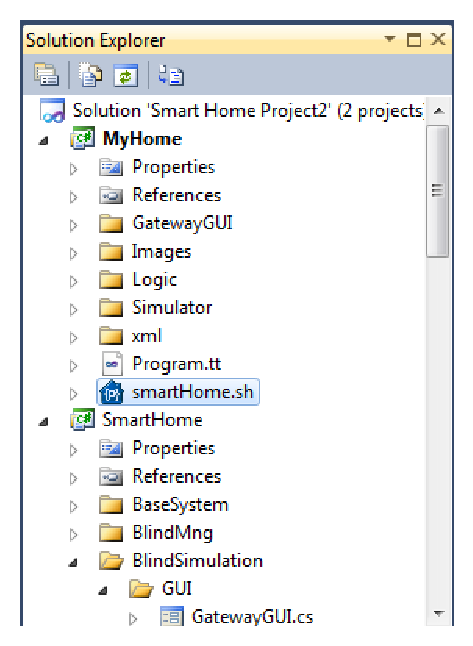
\includegraphics[width=.55\linewidth]{apendixA/images/solutionExplorer.eps}
             \vspace{1cm}
     \end{center} 
\item Ahora tendremos un canvas en el que podemos arrastrar elementos. El fondo blanco representa el hogar inteligente, es decir, todo lo que arrastremos al canvas ser� una nueva caracter�stica del hogar. Para ver los elementos que pueden ser arrastrados, debemos ir a la ventana \emph{Toolbox}, sino est� visible pulsamos en \emph{View}-->\emph{Toolbox}.
    \begin{center}
            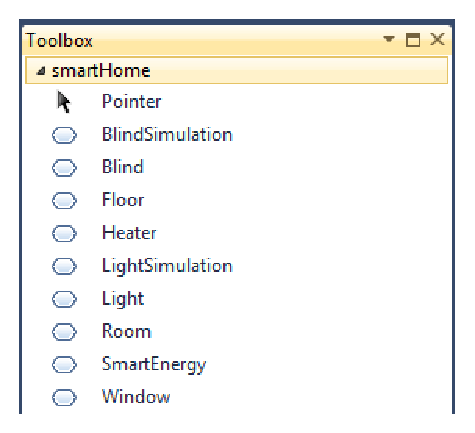
\includegraphics[width=.55\linewidth]{apendixA/images/toolbox.eps}
             \vspace{1cm}
     \end{center} 
\item Los elementos que dependen de otros, como por ejemplo las habitaciones (\emph{Room}) necesitan de una planta (\emph{Floor}), es necesario arrastrarlos encima del elemento del que dependen. De este modo, los elementos \emph{Window}, \emph{Light}, \emph{Heater}, si quieren ser a�adidos, deben ser arrastrados sobre una habitaci�n. Mientras que el elemento \emph{Blind} deber� hacerlo sobre \emph{Window}.
     \begin{center}
            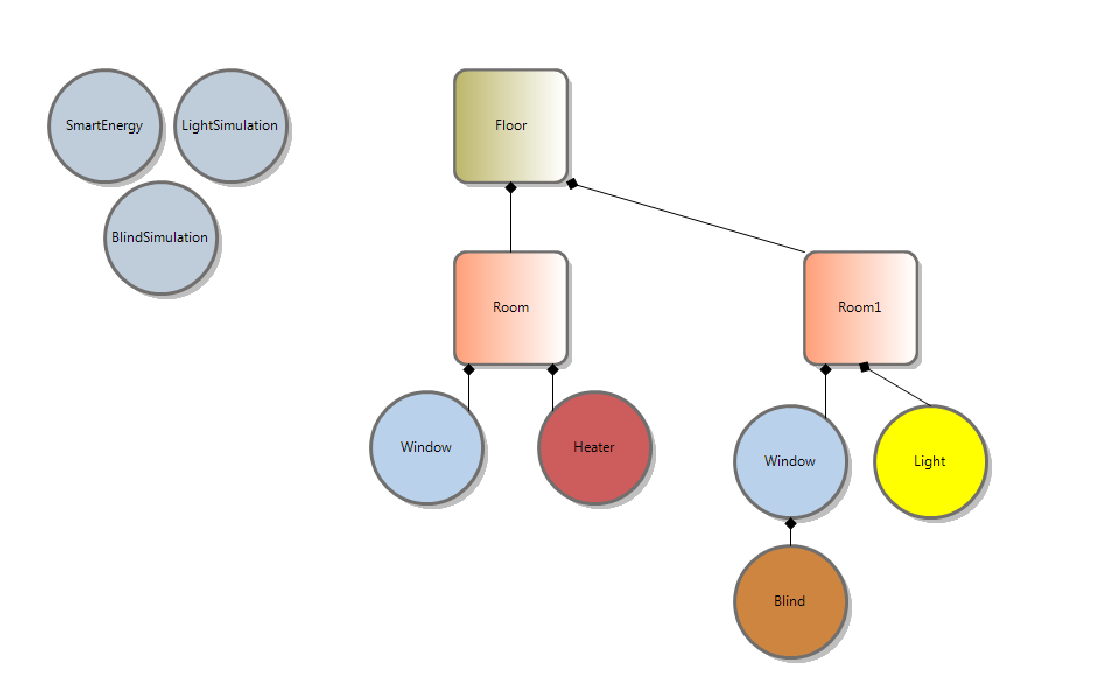
\includegraphics[width=.75\linewidth]{apendixA/images/exampleSmartHome.eps}             
     \end{center} 
\item Cuando tengamos el modelo preparado lo guardamos, y procedemos a generar el c�digo correspondiente para esa configuraci�n. Para ello, desde la ventana \emph{Solution Explorer}, debemos pulsar sobre el bot�n \emph{Transform All Templates}.
    \begin{center}
            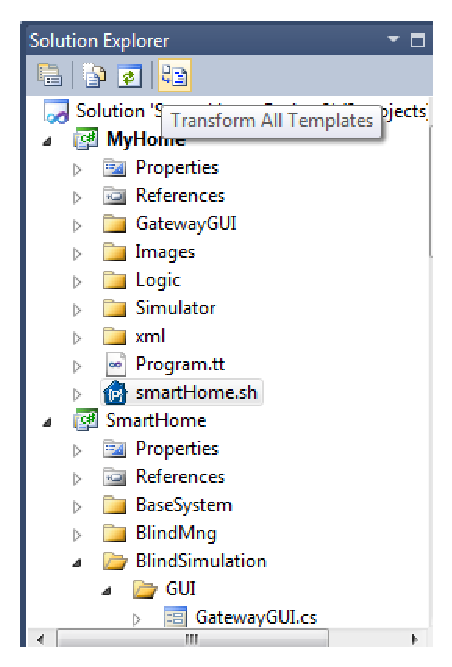
\includegraphics[width=.45\linewidth]{apendixA/images/transformAllTemplates.eps}
             \vspace{1cm}
     \end{center} 
\item Para ejecutar la configuraci�n que hemos creado, hacemos click con el bot�n derecho sobre el proyecto denominado \emph{MyHome} y escogemos \emph{Debug}-->\emph{Start New Instance}
     \begin{center}
            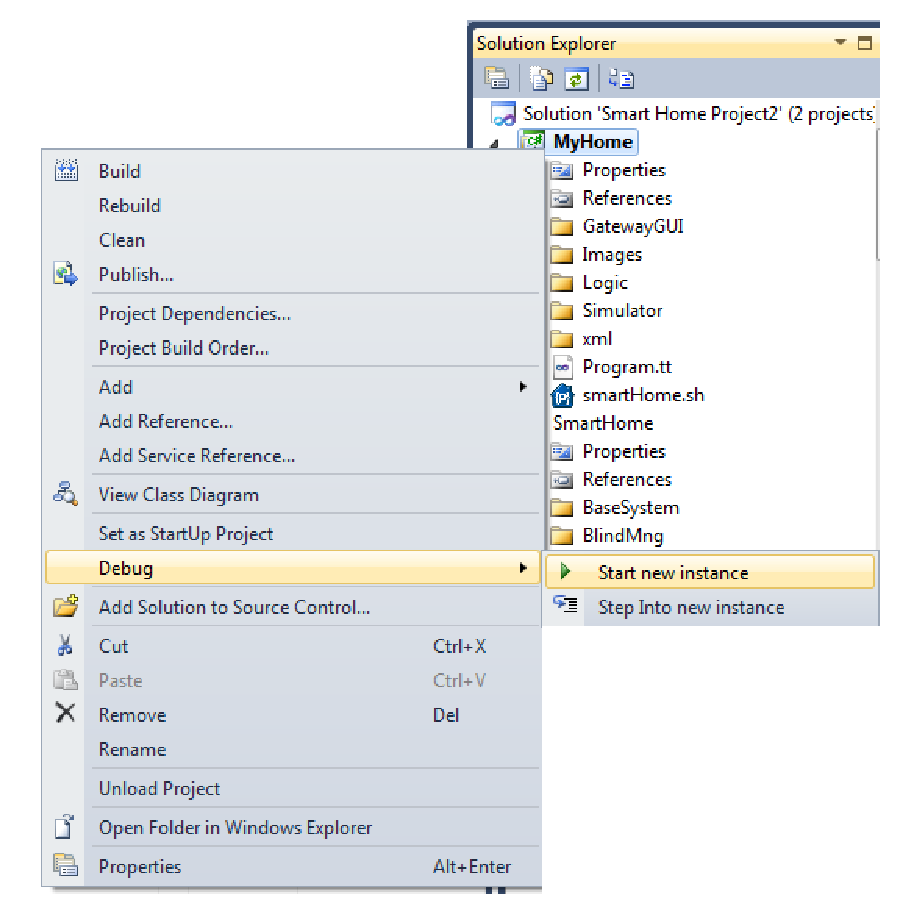
\includegraphics[width=.65\linewidth]{apendixA/images/startNewInstance.eps}
             \vspace{1cm}
     \end{center} 
\end{enumerate}

Existe la posibilidad de que cuando guardemos una configuraci�n nos alerte de alg�n error, si esto sucede, es porque hemos violado alguna de las restricciones que contiene un hogar inteligente, y se nos avisar� de ello en la ventana \emph{Error List}. Por ejemplo, si a�adimos la caracter�stica \emph{SmartEnergy}, sin que en ninguna de las habitaciones exista un calefactor y una ventana, se producir� un error por crear un modelo inv�lido.
  \begin{center}
            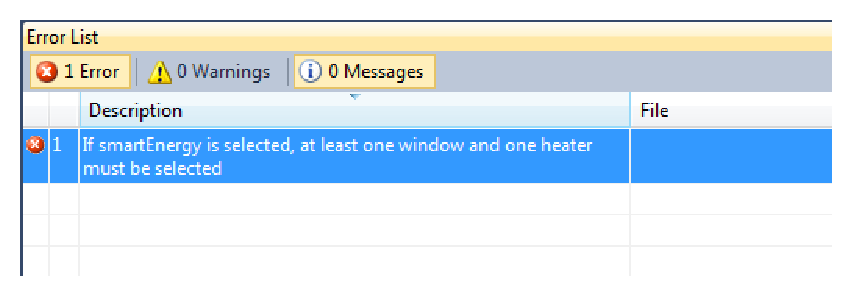
\includegraphics[width=.55\linewidth]{apendixA/images/error.eps}
             \vspace{1cm}
  \end{center}

 % Appendix I

% CONFIG: Bibliography style
\cleardoublepage                            % start in right side page
\addcontentsline{toc}{chapter}{Referencias}  % add this "chapter" to the ToC, with the name "Bibliography"
%pohl:2005\bibliographystyle{alpha}                  % bibliography style
%clements:2002\bibliographystyle{alpha}
%batory:2004\bibliographystyle{alpha}
%albahari:2010\bibliographystyle{alpha}
%\bibliographystyle{abbrv}                  % bibliography style
\bibliographystyle{alpha}

\bibliography{references/pfc}

\end{document}
